\section{Chemins du sud}

25 nov. 2010

\begin{multicols}{2}

Salut à vous ! Encore quelques nouvelles de moi, histoire de vous montrer de belles photos..

Tout d'abord je ne vous ai pas parlé de la notion de temps ici, cela semble pourtant important pour mieux comprendre ce qui s'est passé ces derniers jours. L'art de vivre ici se résume en deux mots : mora mora, ce qui se traduit par faire les choses, mais lentement, ne pas s'énerver (qui a dit que j'ai bien choisi le pays ?). C'est vrai que ça a des bons cotés, mais lorsqu'on est dans les transports c'est plus galère. Commençons par le taxi brousse : il s'agit d'un mini van style volkswagen ou toyota (capacité usine : 9 places) dans lequel on a ajouté une rangée de sièges entre chacune déjà présente. Un taxi brousse normal se retrouve avec une capacité d'environs 25 personnes (30 des fois) et des galeries sur le toit pouvant acceuillir 500kg de riz, ou des velos, des socs de charues, des sacs de voyage, des animaux.. ou un ensemble de tout à la fois. Une fois que l'on a défini ce qu'est un taxi brousse, vient maintenant son trajet. Le taxi brousse ne part que quand il est plein (sauf rares occasions) et rien ne l'empêche de s'arrêter plusieurs heures en milieu de trajet, voire de vous balancer dans un autre taxi brousse car il a décidé qu'il ne finirait pas le trajet, malag' style ! Ce transport nécessite donc une bonne dose de patience, je pense en fait que l'on est prêt à le prendre lorsqu'on s'est habitué au fatalisme de l'île, lorsque plus rien n'est étonnant, alors ça peut même être agréable (si si !). C'est avec ce mode de transport, le moins cher qu'il soit, que j'avais quitté la capitale vers Antsirabe, puis Fianar et de Malakar vers Ambalavao et Ranohira.

Je vous ai quitté à Ranohira où j'avais rendez vous avec Michel, guide touristique qui allait prendre des clients à Fort Dauphin et m'a proposé de monter avec lui et Harrys, le chauffeur et mécano du 4x4 en échange de financer une partie de l'essence. C'est donc parti pour deux jours de 4x4 en mode Paris-Dakar dans le grand sud de l'île. Nous sommes partis de Ranohira puis sommes passés à Tuléar puis cap sur la route du sud, 700km de piste cotière magnifique. Voici donc quelques instants de cette magnifique route.. en commençant par un caméléon de toute beauté qui a pris la pause comme une star.

\smallbreak
\hspace*{-0.65cm}
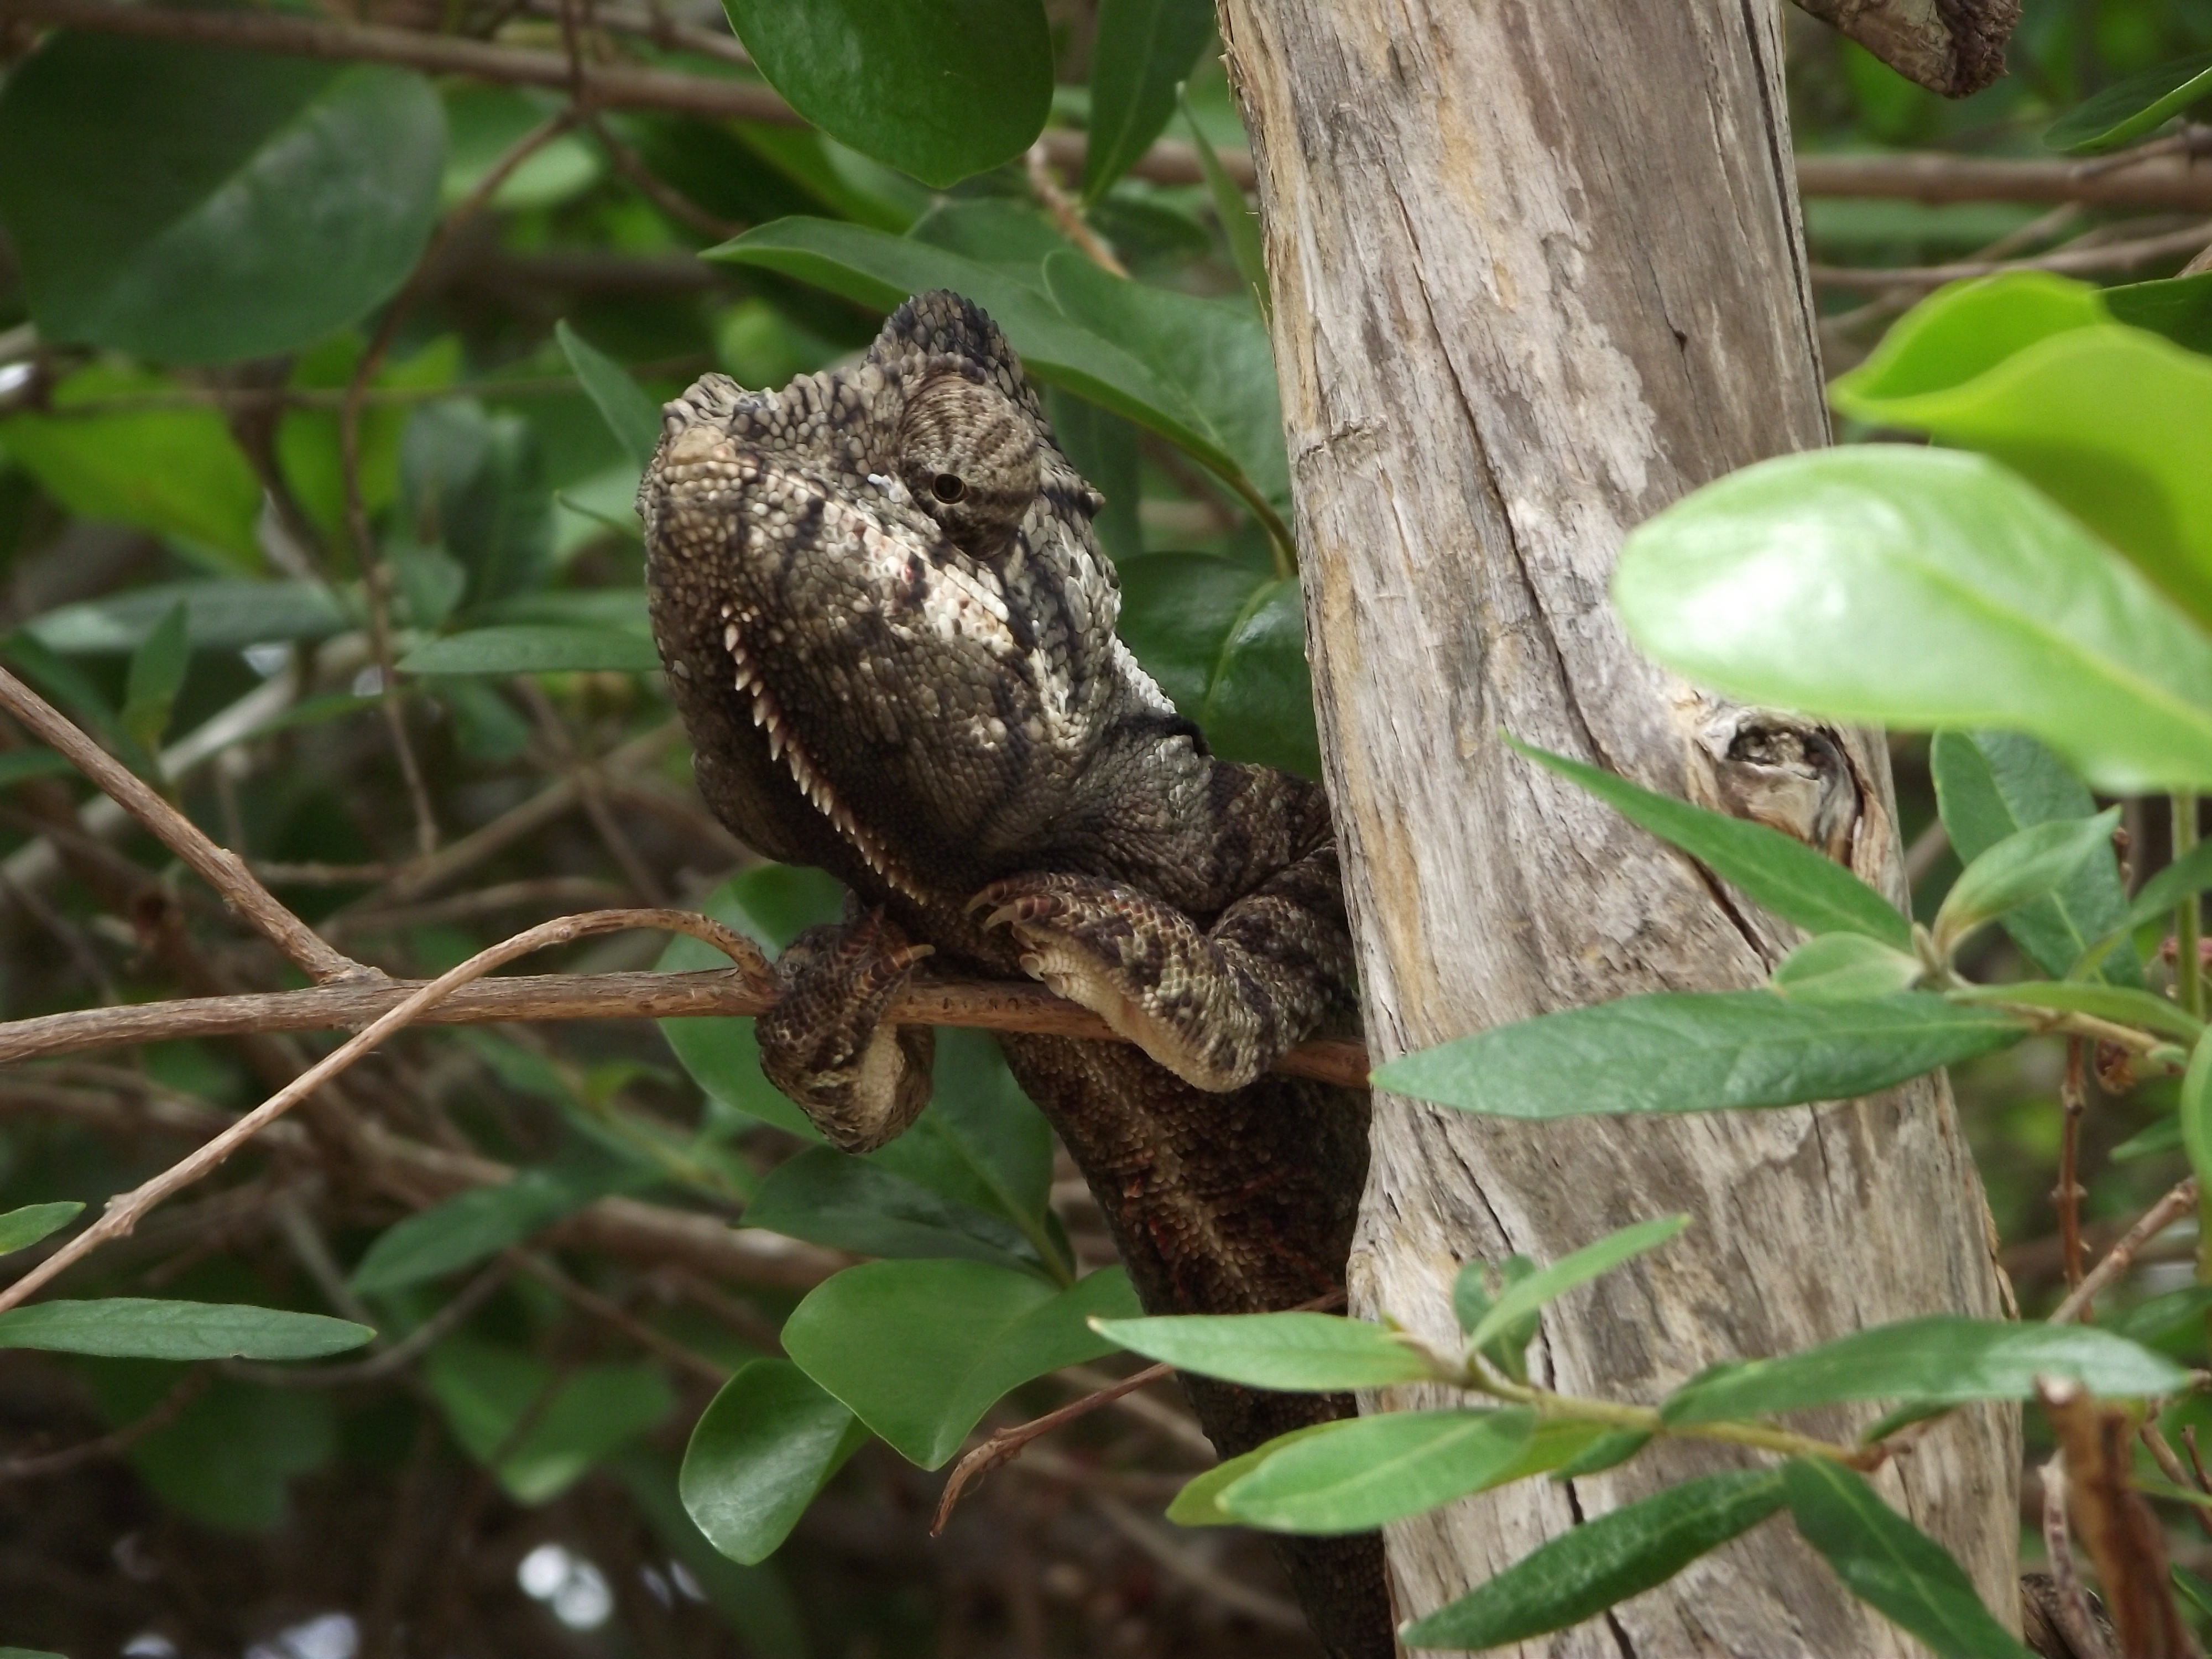
\includegraphics[width=5cm]{articles/Chemins-du-sud/DSCF0291.JPG}
\smallbreak

Ici des grandes étendues sèches parsemées de grosses termitières rendent le paysage assez spécial et le sol sans doute peu fertile.

\smallbreak\smallbreak
\hspace*{-0.65cm}
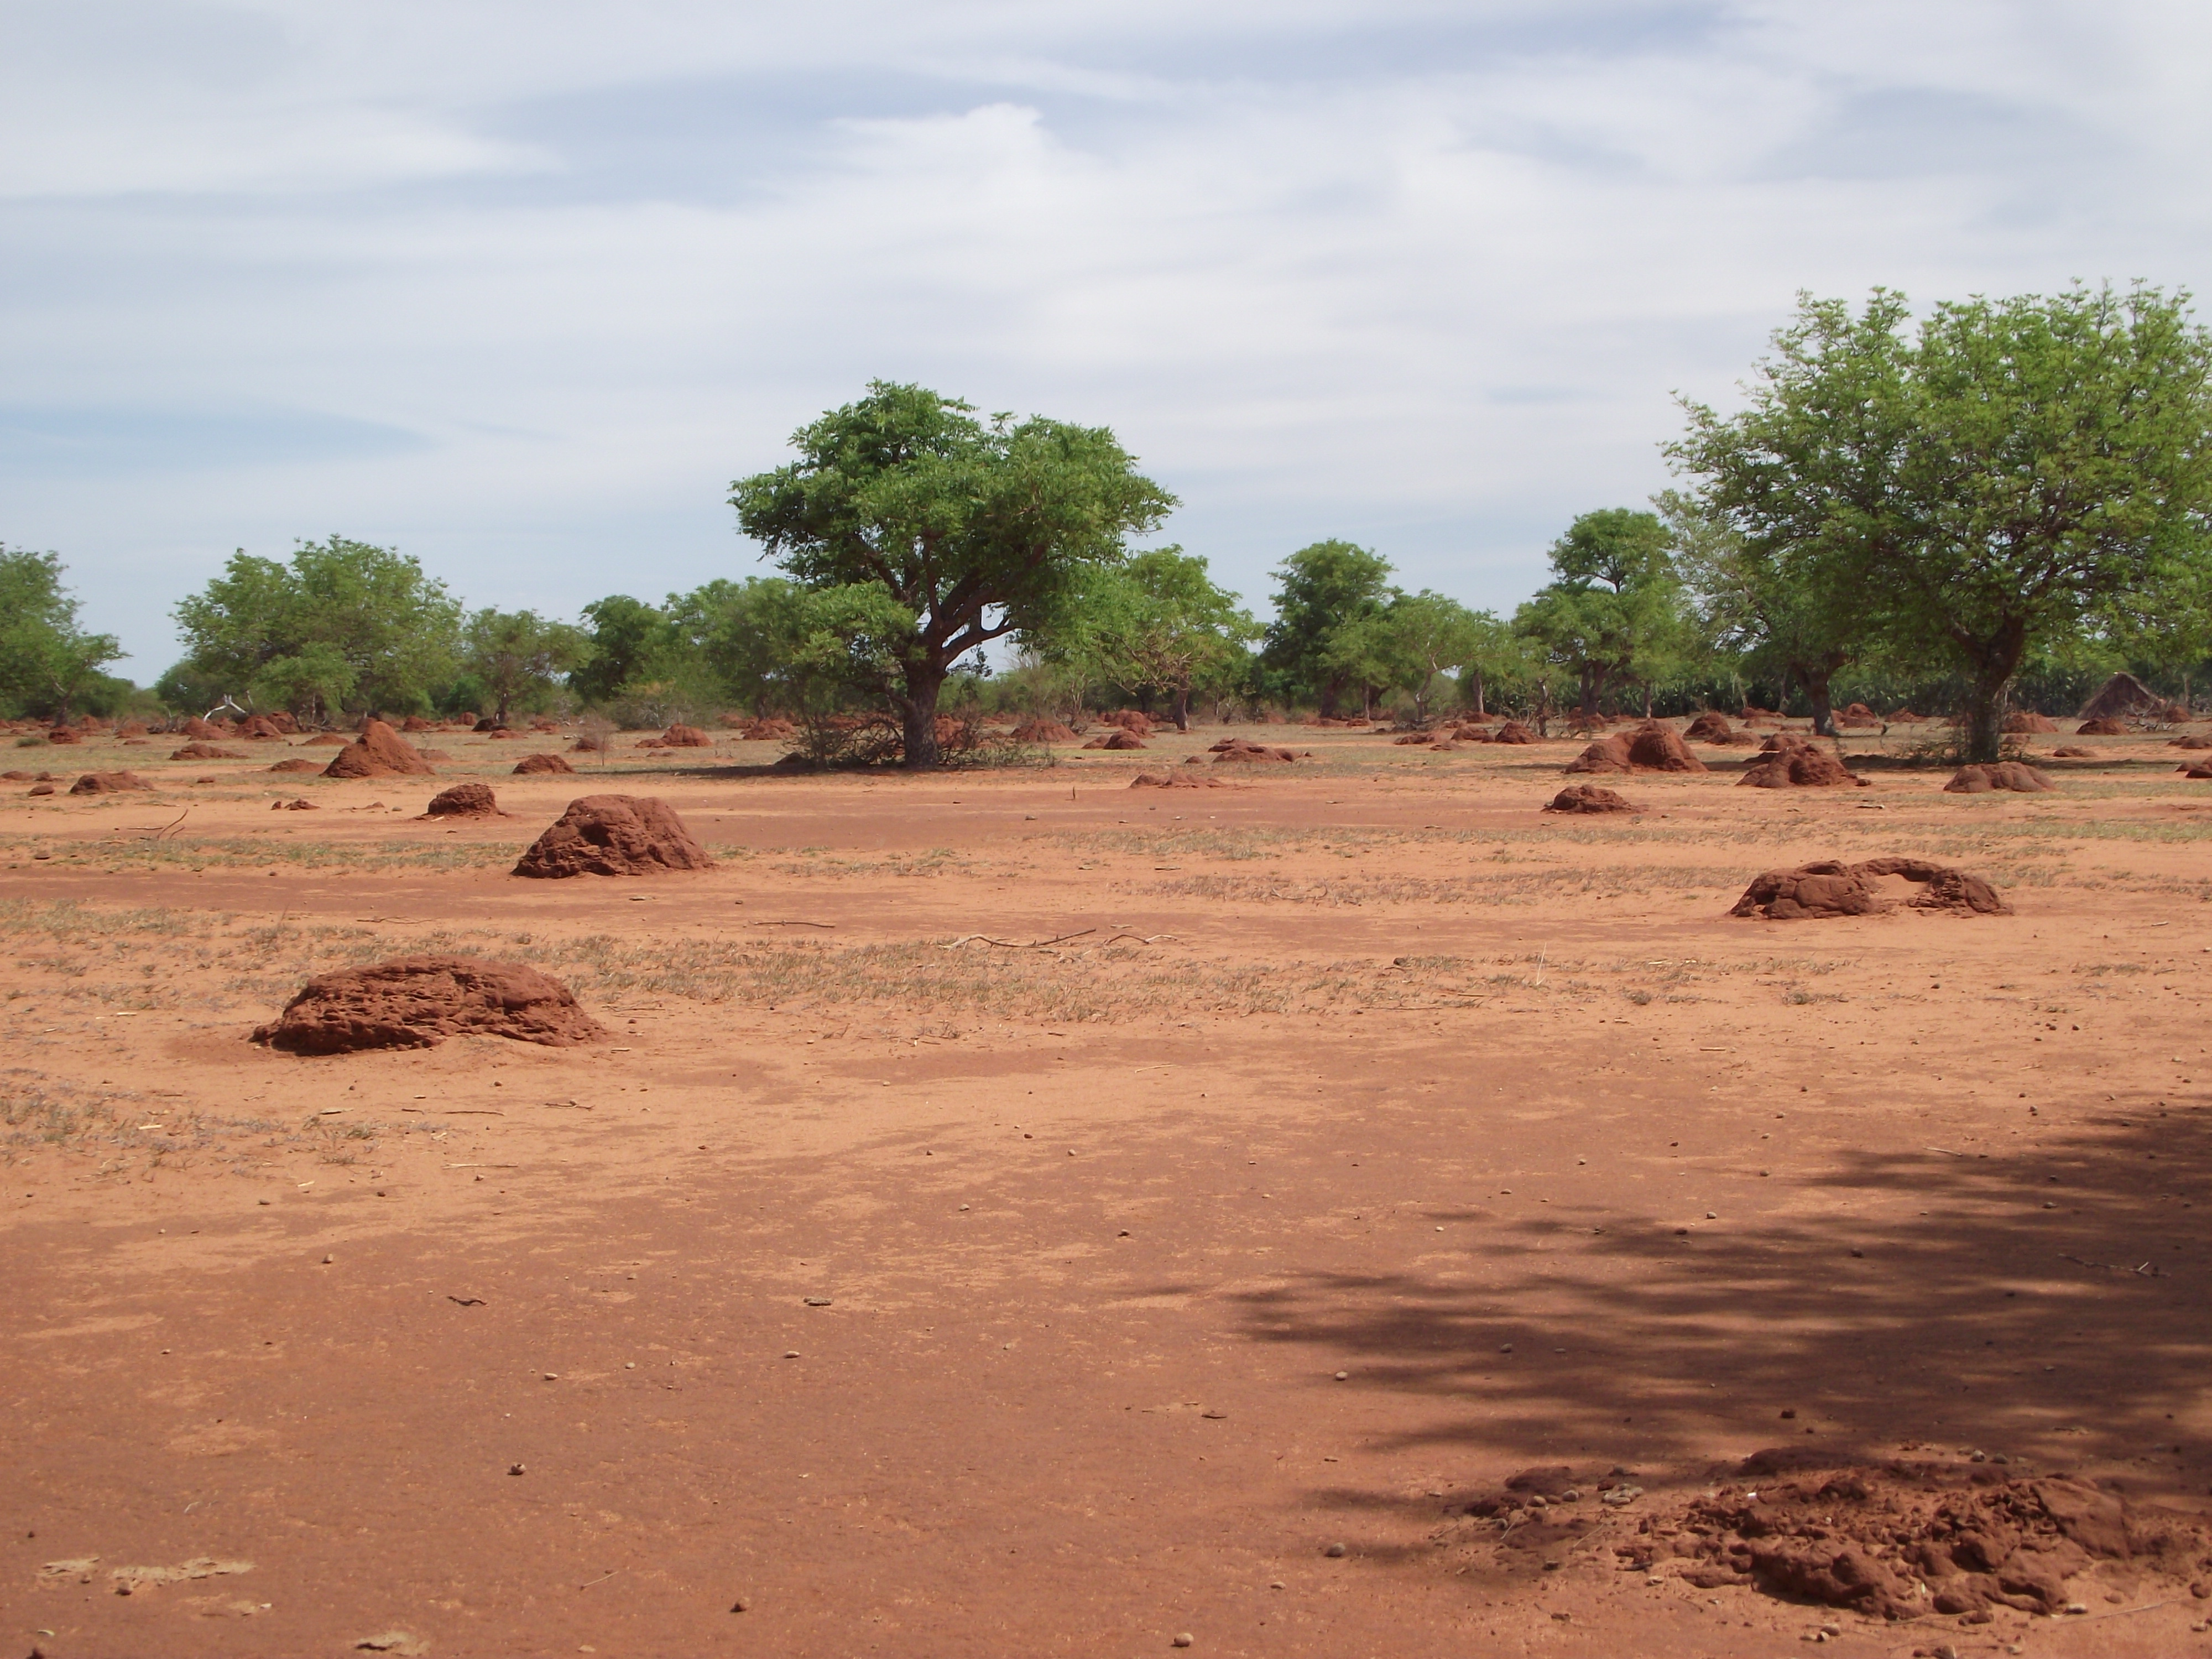
\includegraphics[width=5cm]{articles/Chemins-du-sud/DSCF0299.JPG}
\smallbreak

La traversée d'un village, où la vue d'un vazaha fait venir plein d'enfants en quelques secondes, c'est assez impressionnant. D'autant plus qu'en dehors des villages certaines personnes isolées (femmes ou enfants en général) partaient se cacher en courant en voyant un blanc dans le 4x4. Je n'y croyais pas mais Michel m'a confirmé que certaines ethnies malgache ont peur des blancs, le phénomène s'atténue dans les villages où l'effet de groupe redonne la confiance.

\smallbreak\smallbreak
\hspace*{-0.65cm}
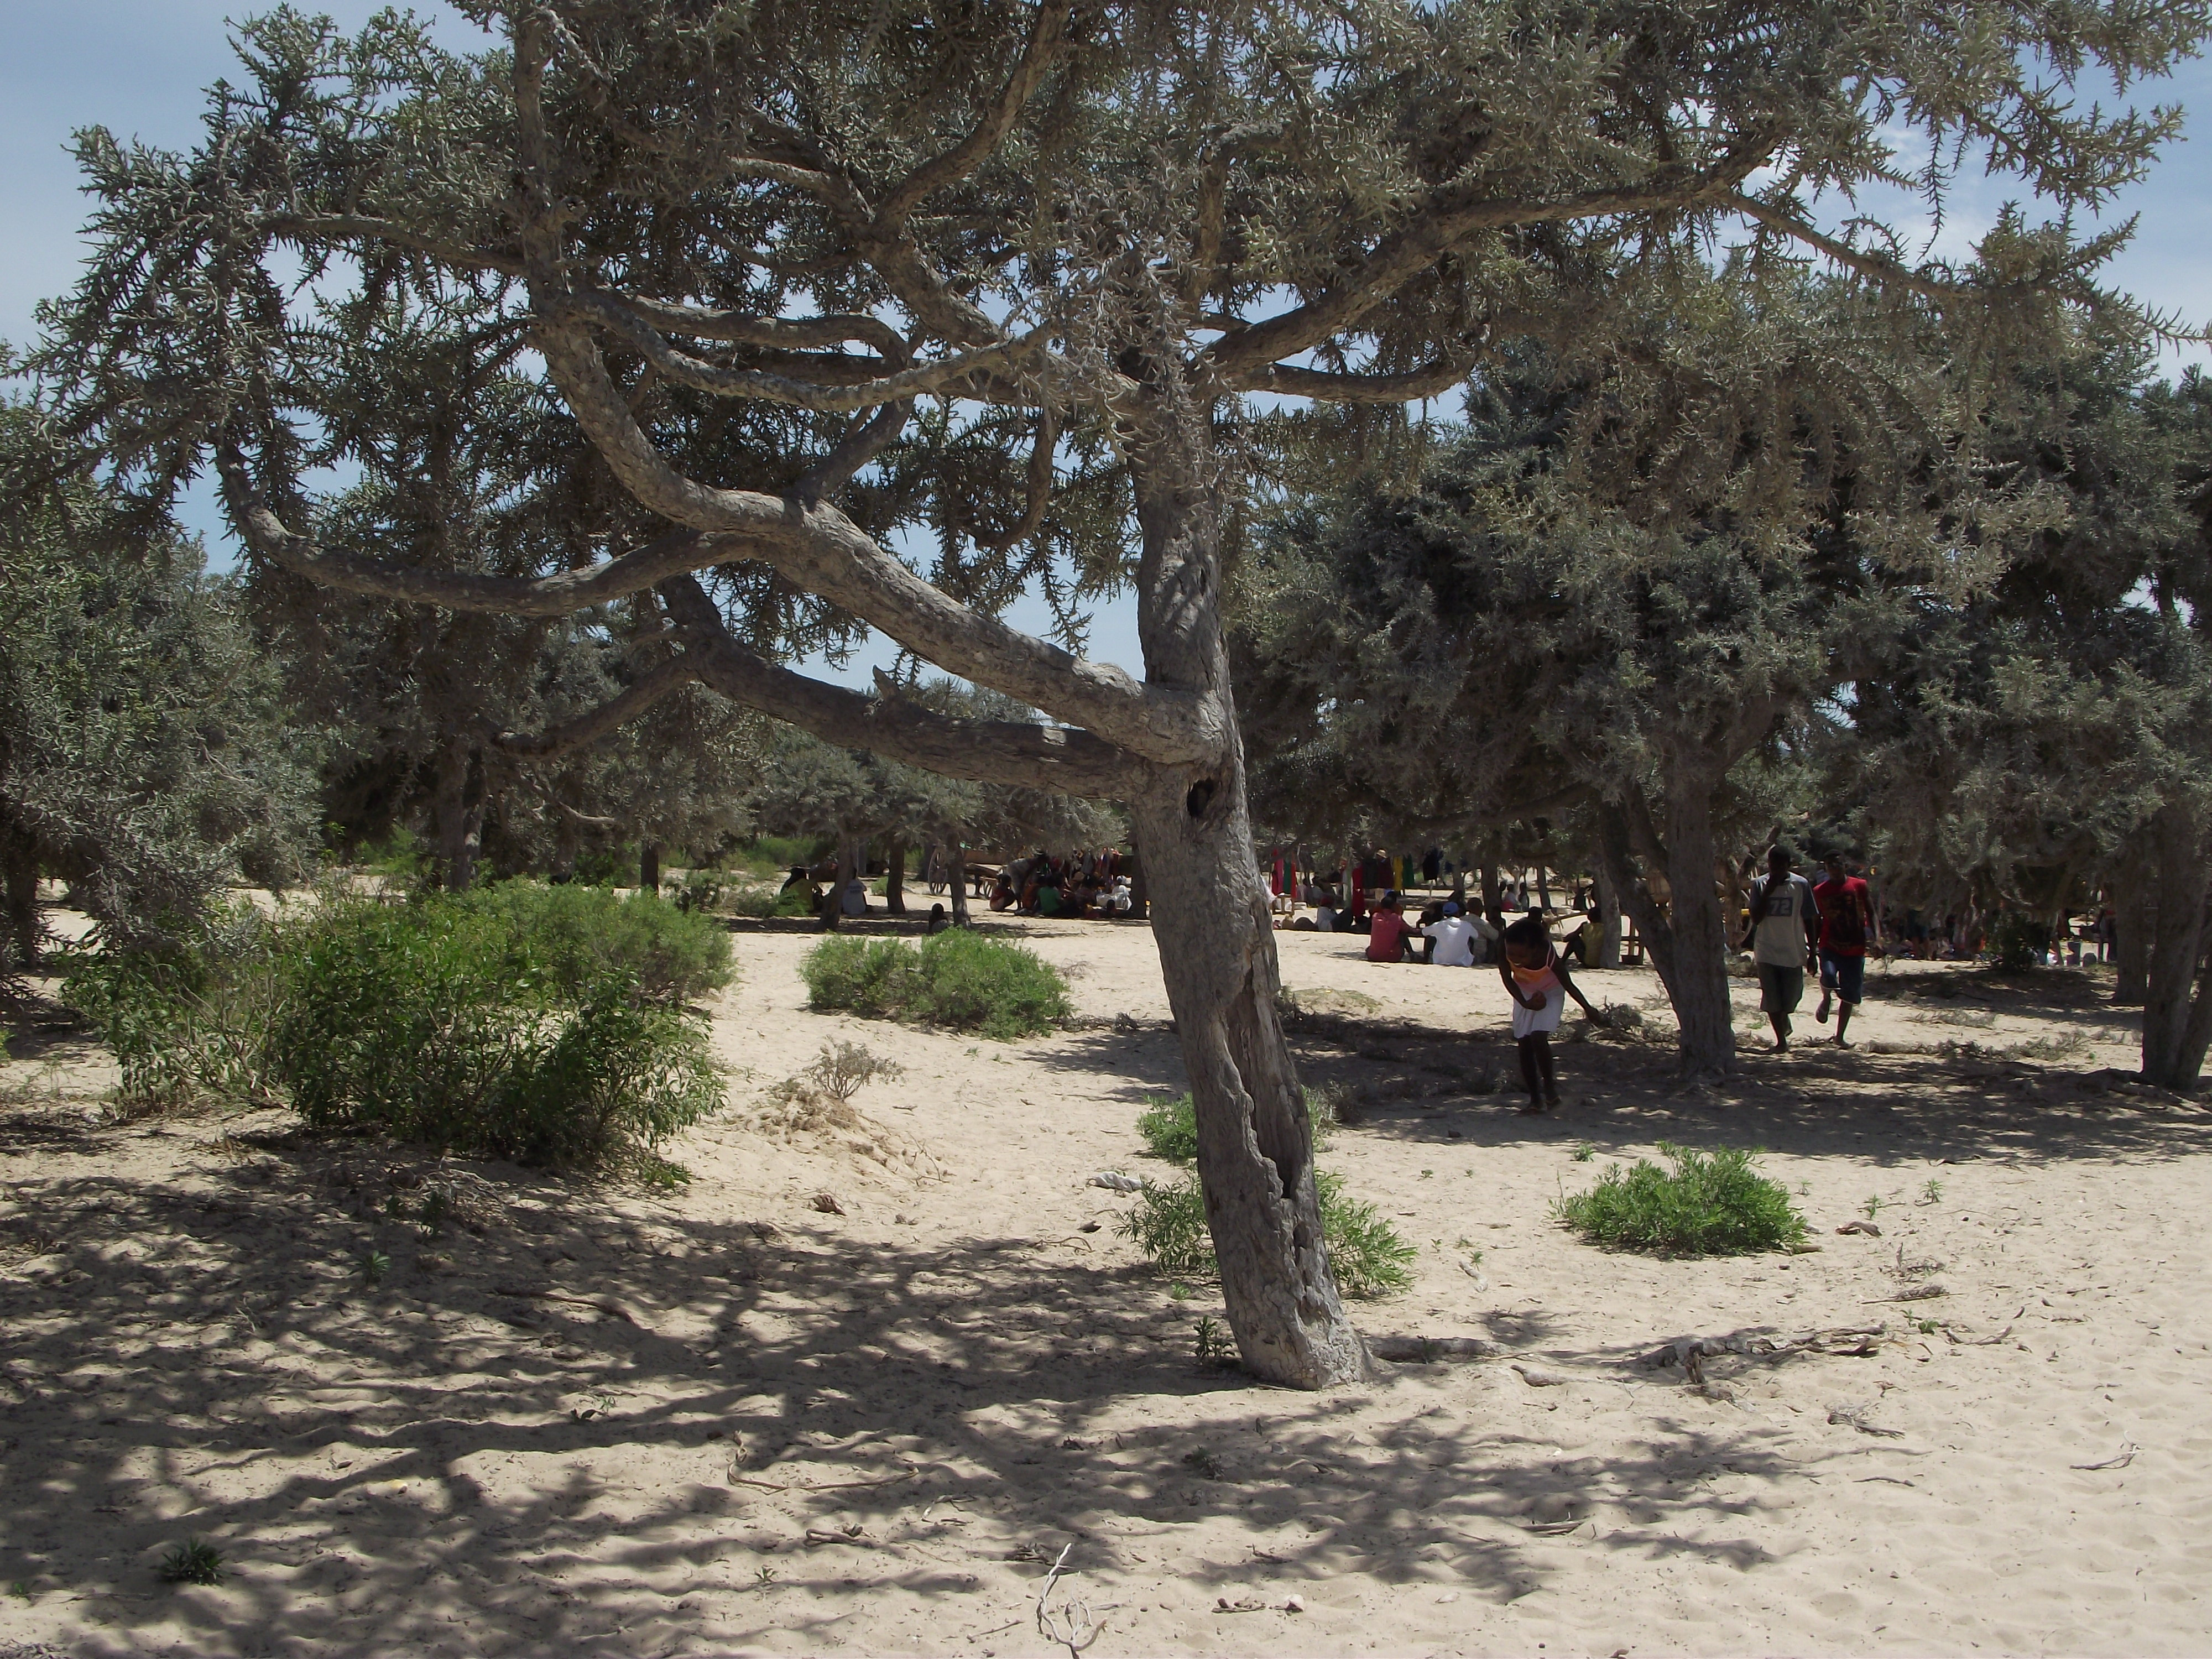
\includegraphics[width=5cm]{articles/Chemins-du-sud/DSCF0303.JPG}
\smallbreak

Allez, on commence les images de la côte.. Je vous préviens que vu la beauté de cette côte et mon rapport à la mer vous n'avez pas fini d'en voir. Ici un petit village traversé.

\smallbreak\smallbreak
\hspace*{-0.65cm}
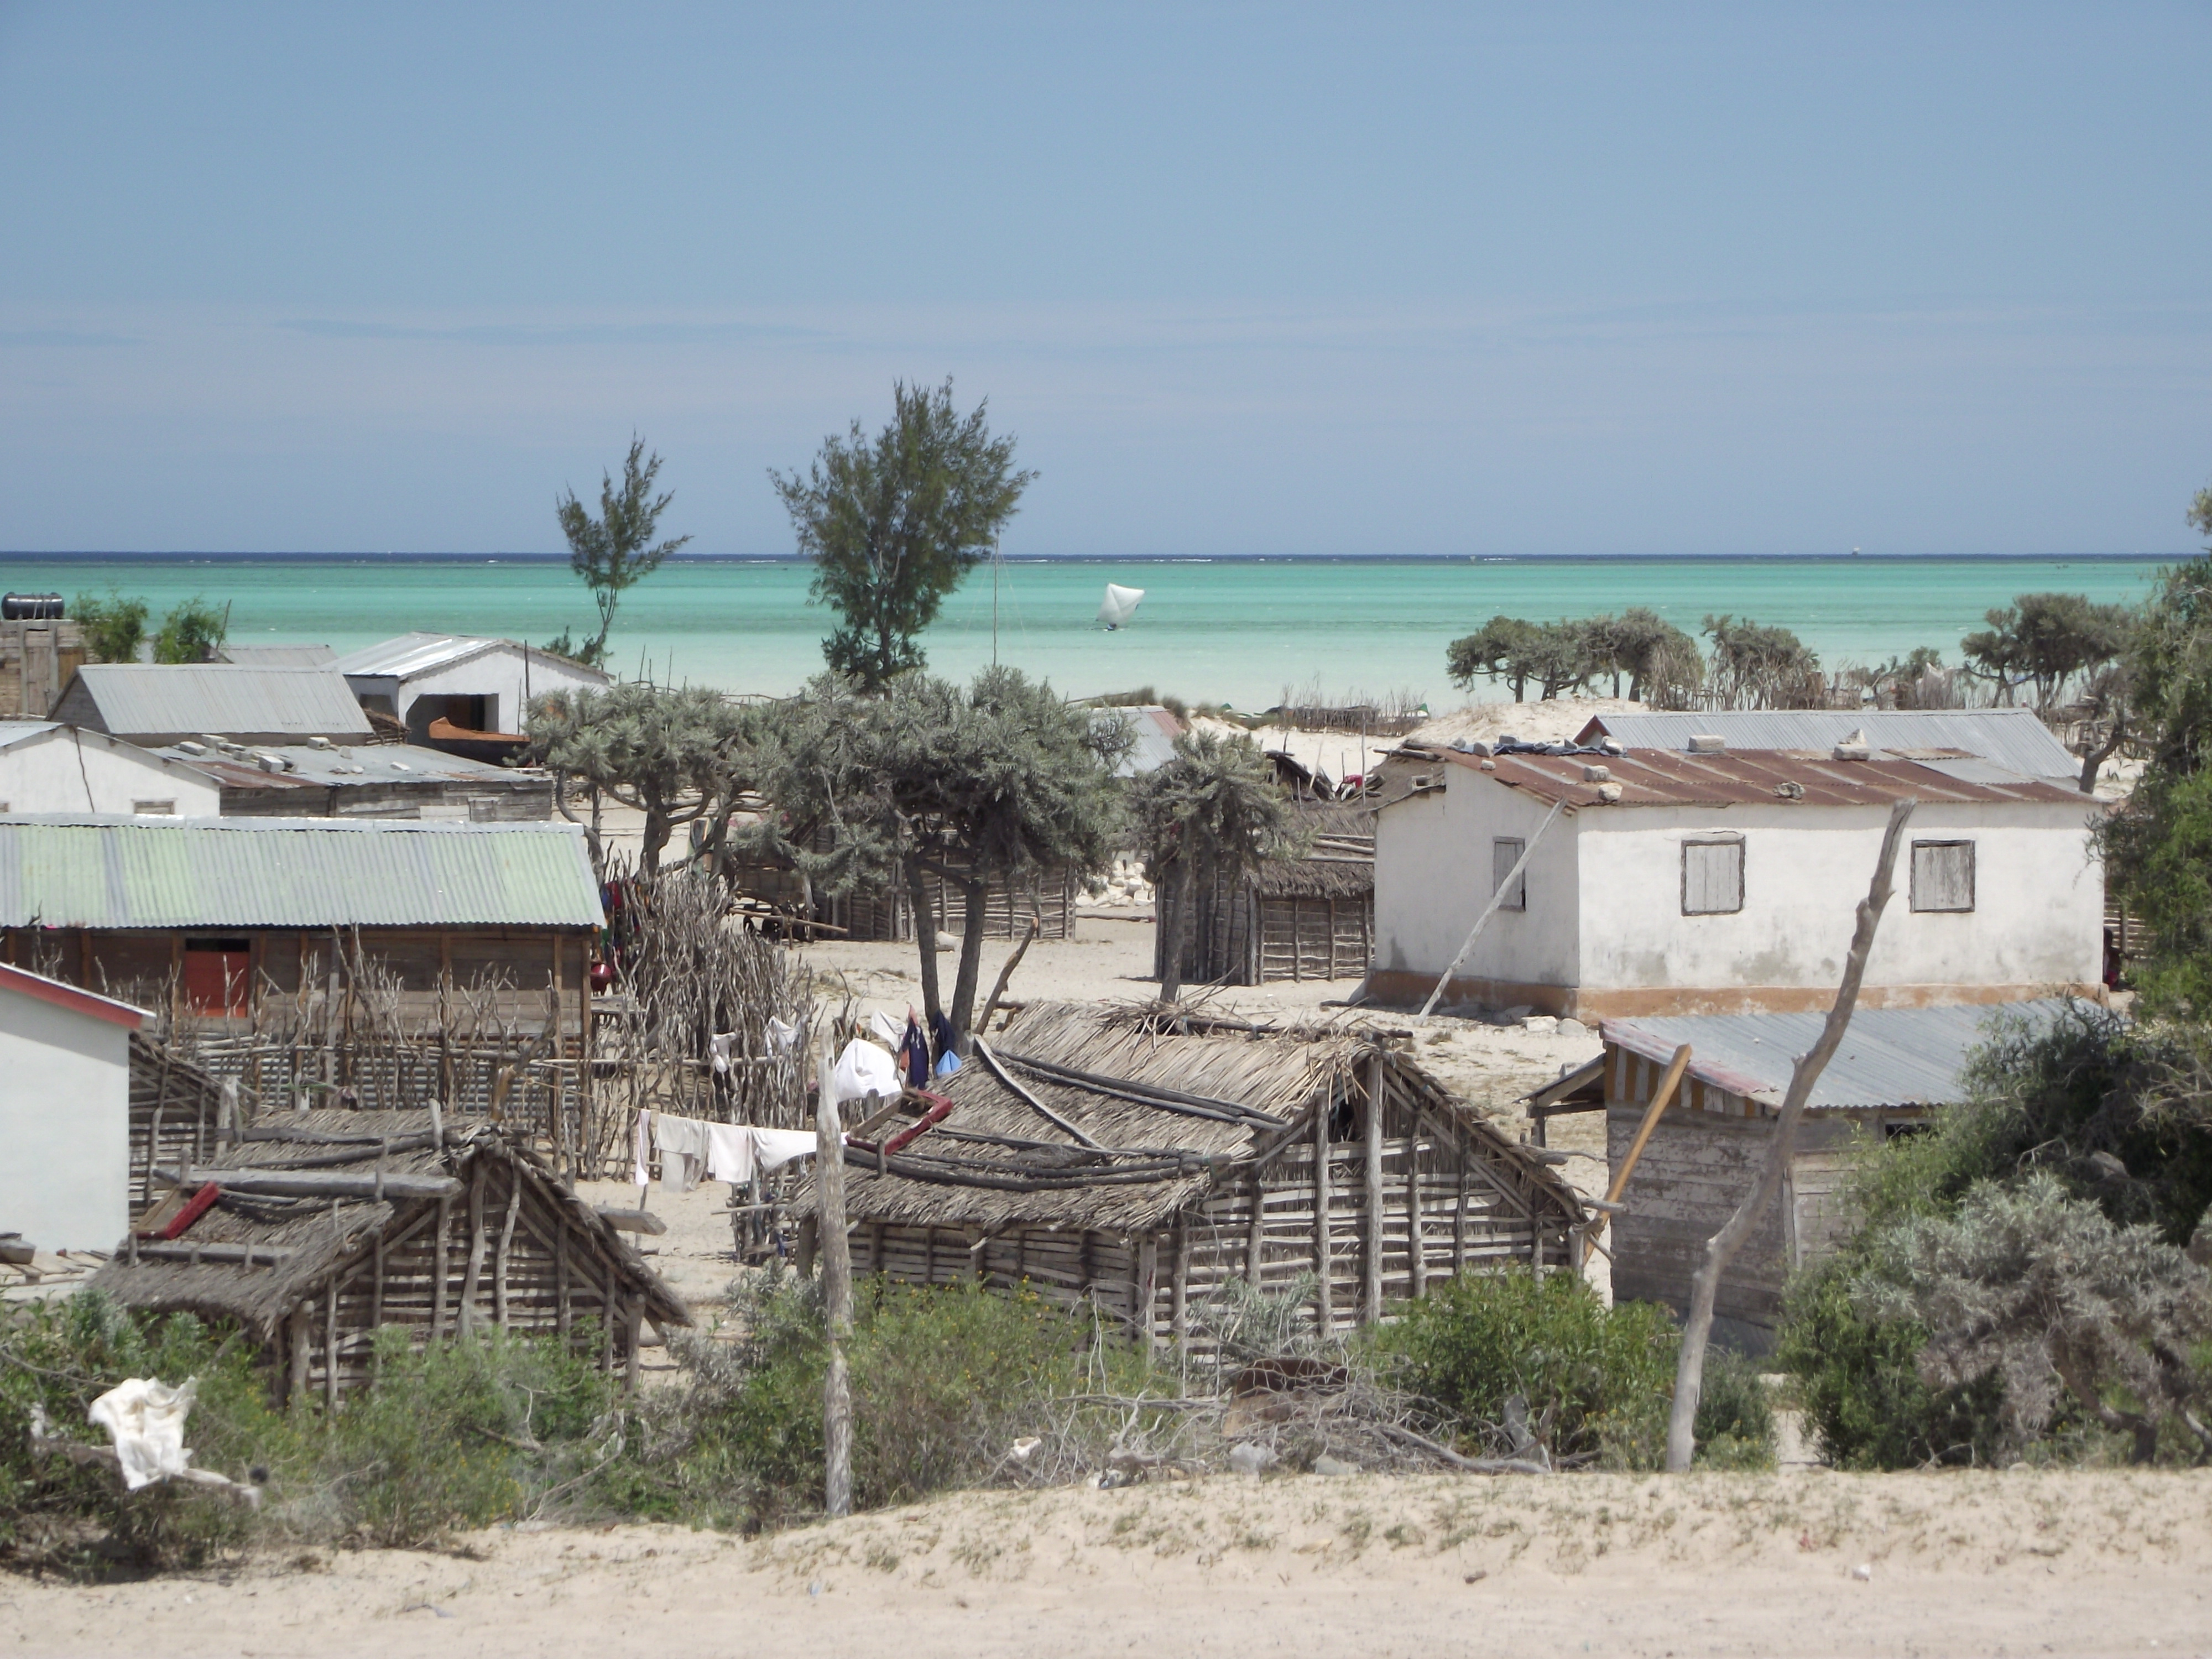
\includegraphics[width=5cm]{articles/Chemins-du-sud/DSCF0306.JPG}
\smallbreak

Puis nous nous sommes arrêtés chez Paola et son papa pour manger un petit rouget grillé que les pêcheurs avaient pris dans leurs filets le matin. On dit bonjour à Paola, toute timide..

\smallbreak\smallbreak
\hspace*{-0.65cm}
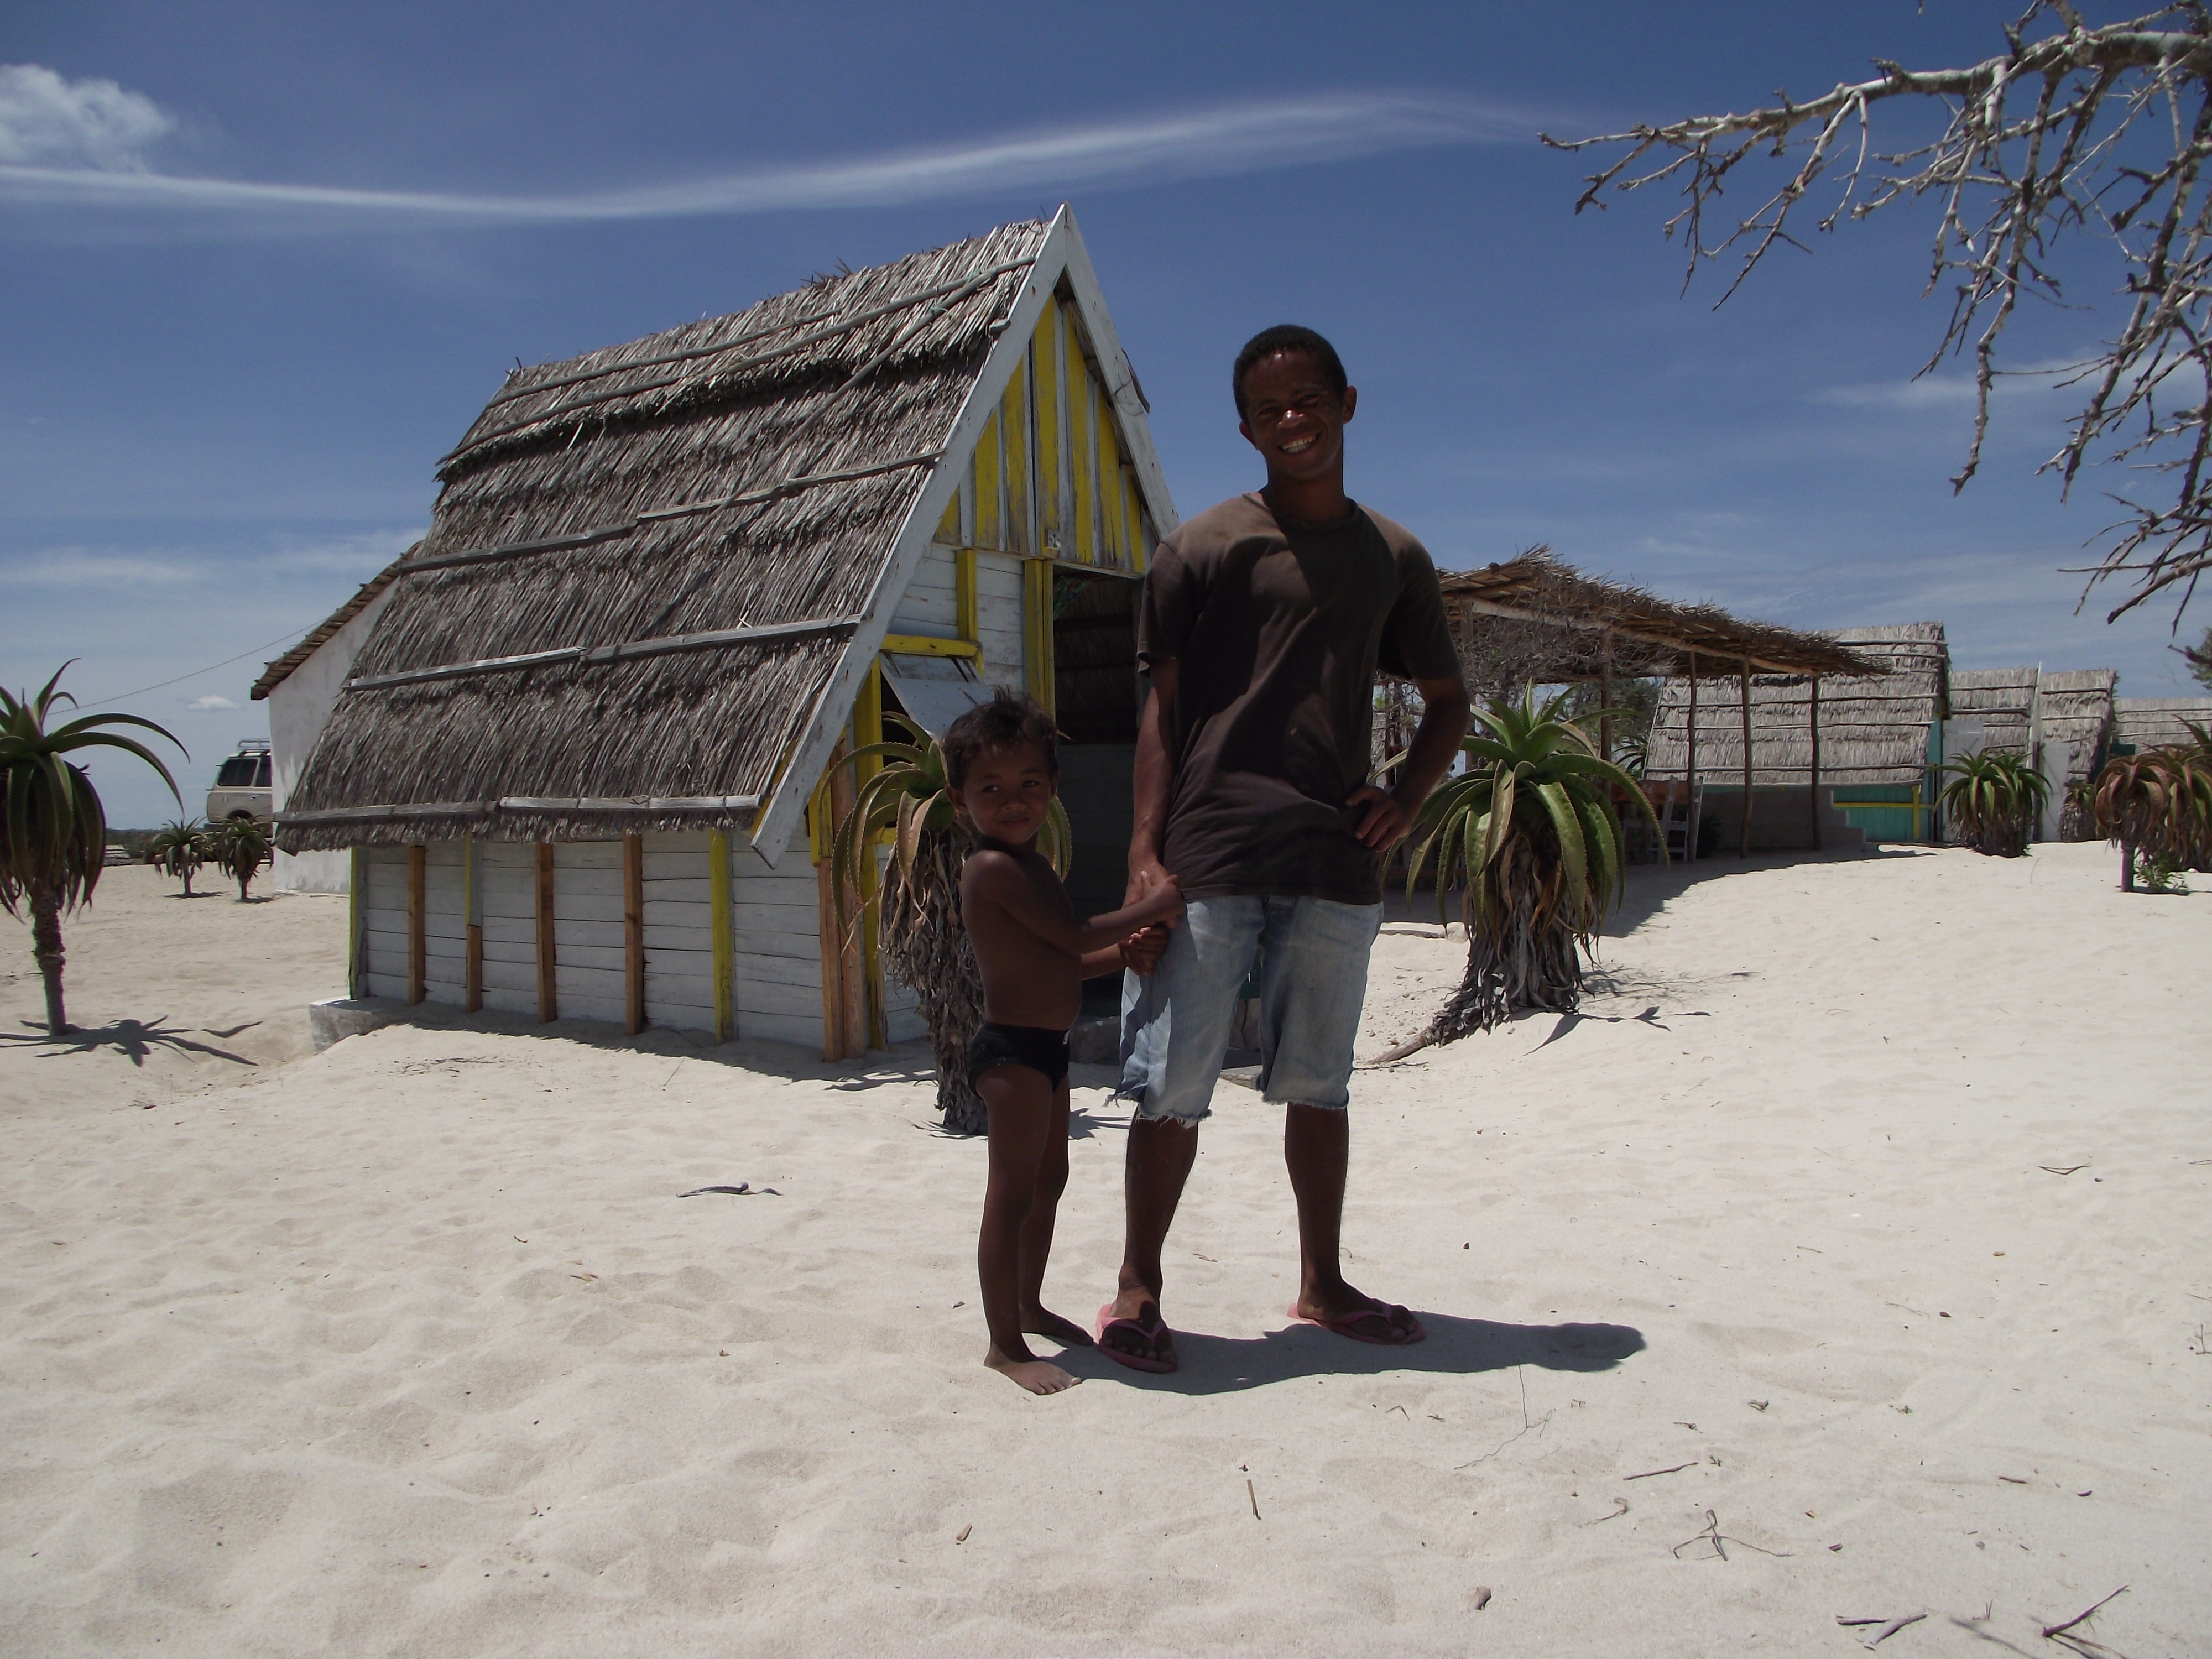
\includegraphics[width=5cm]{articles/Chemins-du-sud/DSCF0310.JPG}
\smallbreak

Ah oui, je vous ai pas montré la table du resto, la classe non ?

\smallbreak\smallbreak
\hspace*{-0.65cm}
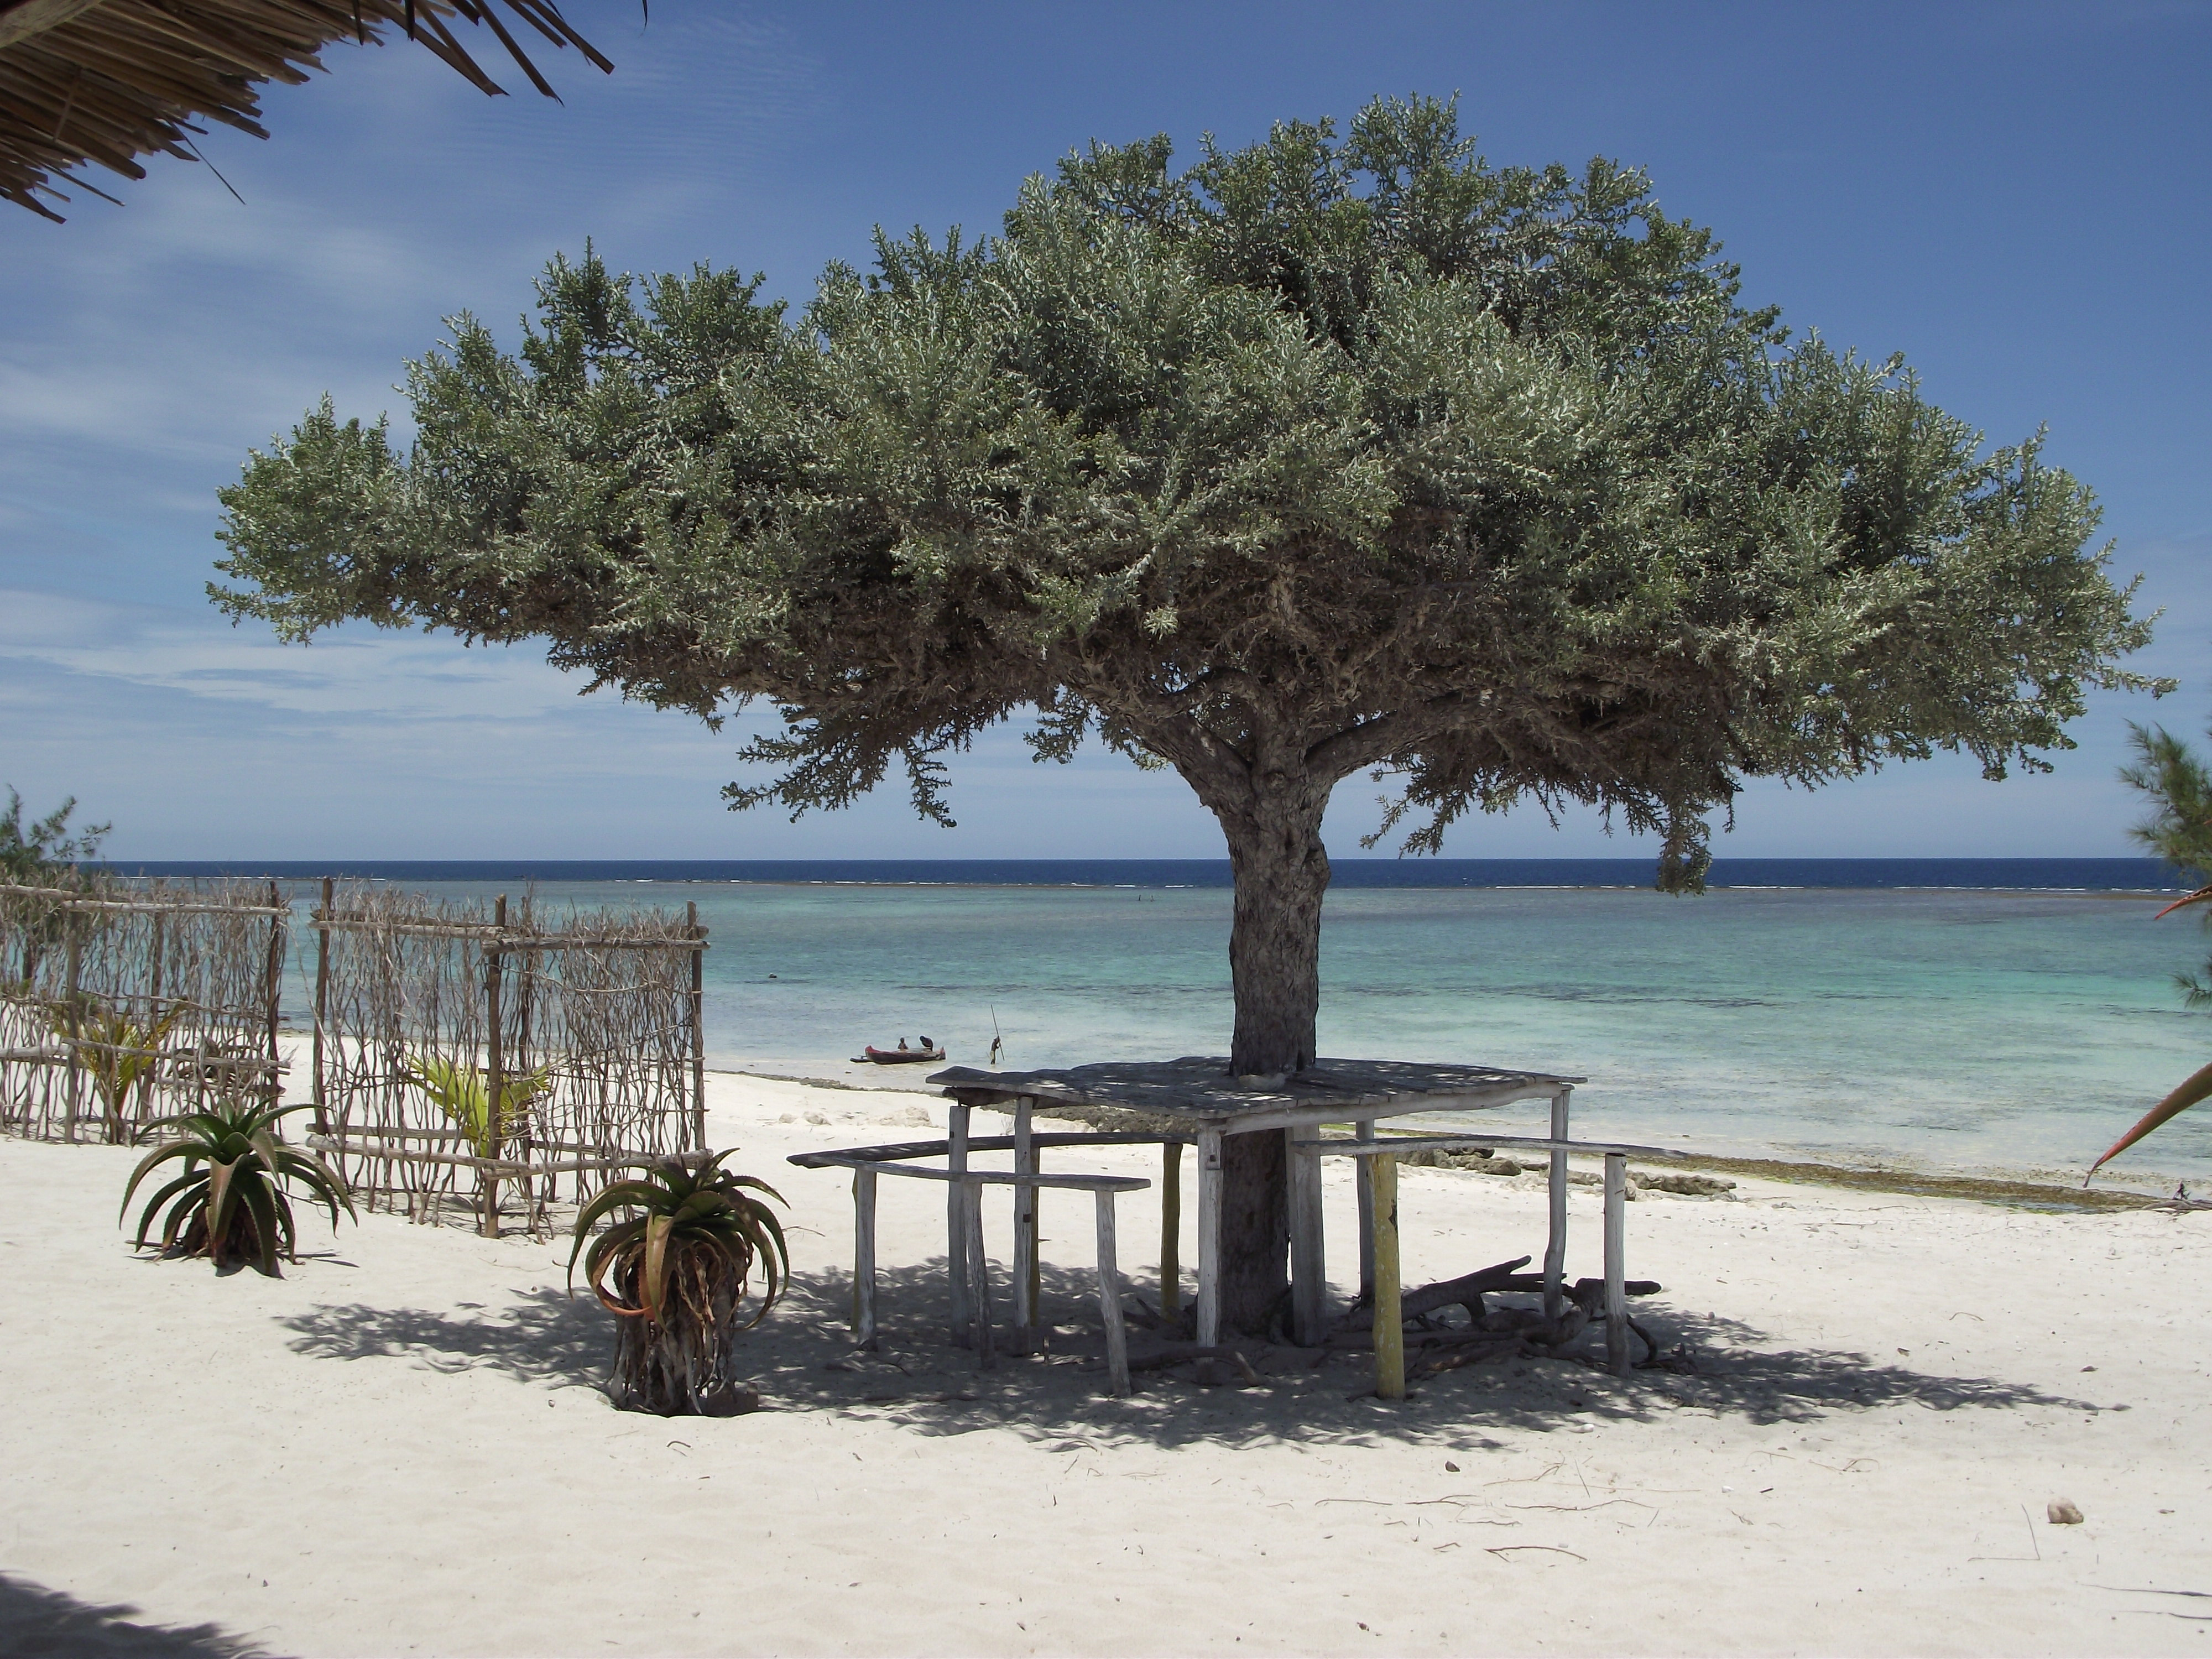
\includegraphics[width=5cm]{articles/Chemins-du-sud/DSCF0316.JPG}
\smallbreak

Spécial dédicace aux pêcheurs grâce à qui on a dégusté ces bons poissons grillés, j'aurais bien été faire un tour sur leur pirogue moi, rien que pour tester si mes notions de voile s'appliquent à ce genre d'embarcation.. affaire à suivre dans le Nord, plus tard dans le voyage.

\smallbreak\smallbreak
\hspace*{-0.65cm}
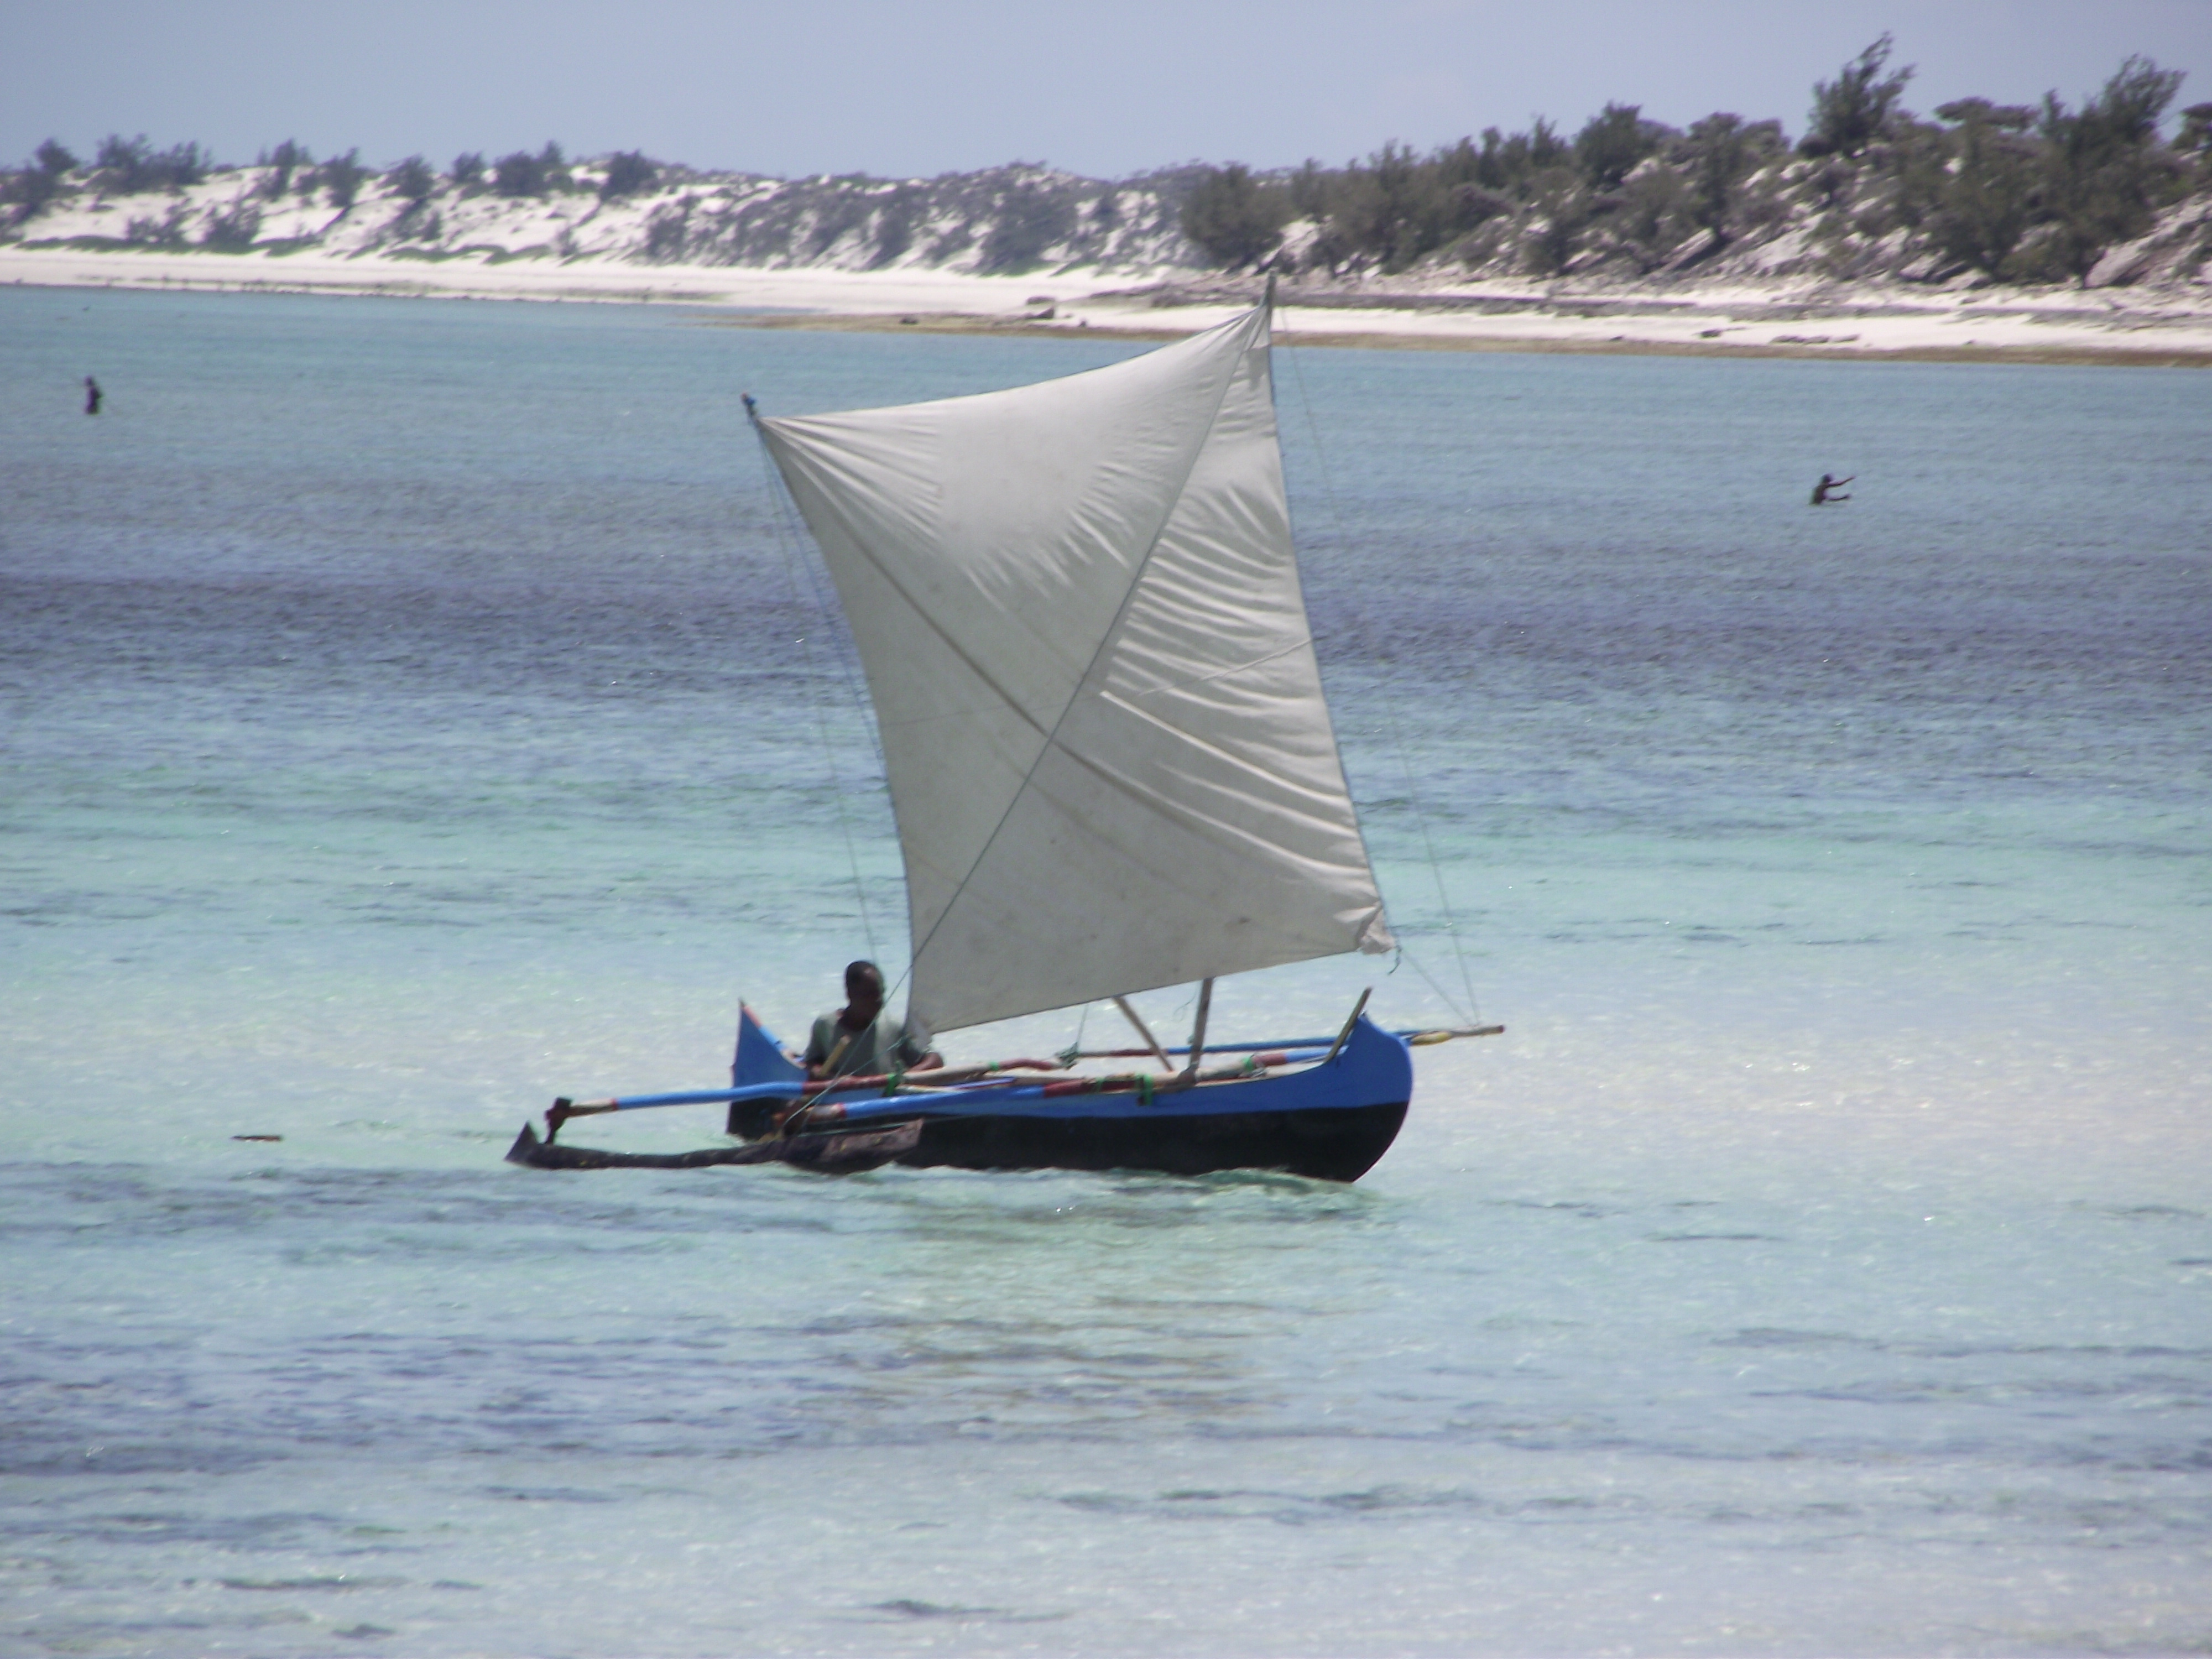
\includegraphics[width=5cm]{articles/Chemins-du-sud/DSCF0319.JPG}
\smallbreak

Puis c'est la séance photo, Harrys notre super chauffeur buvant une THB bien méritée (C'est le genre de bonhomme capable de conduire 34h en l'espace de 48h ! et de la piste qui plus est !).

\smallbreak\smallbreak
\hspace*{-0.65cm}
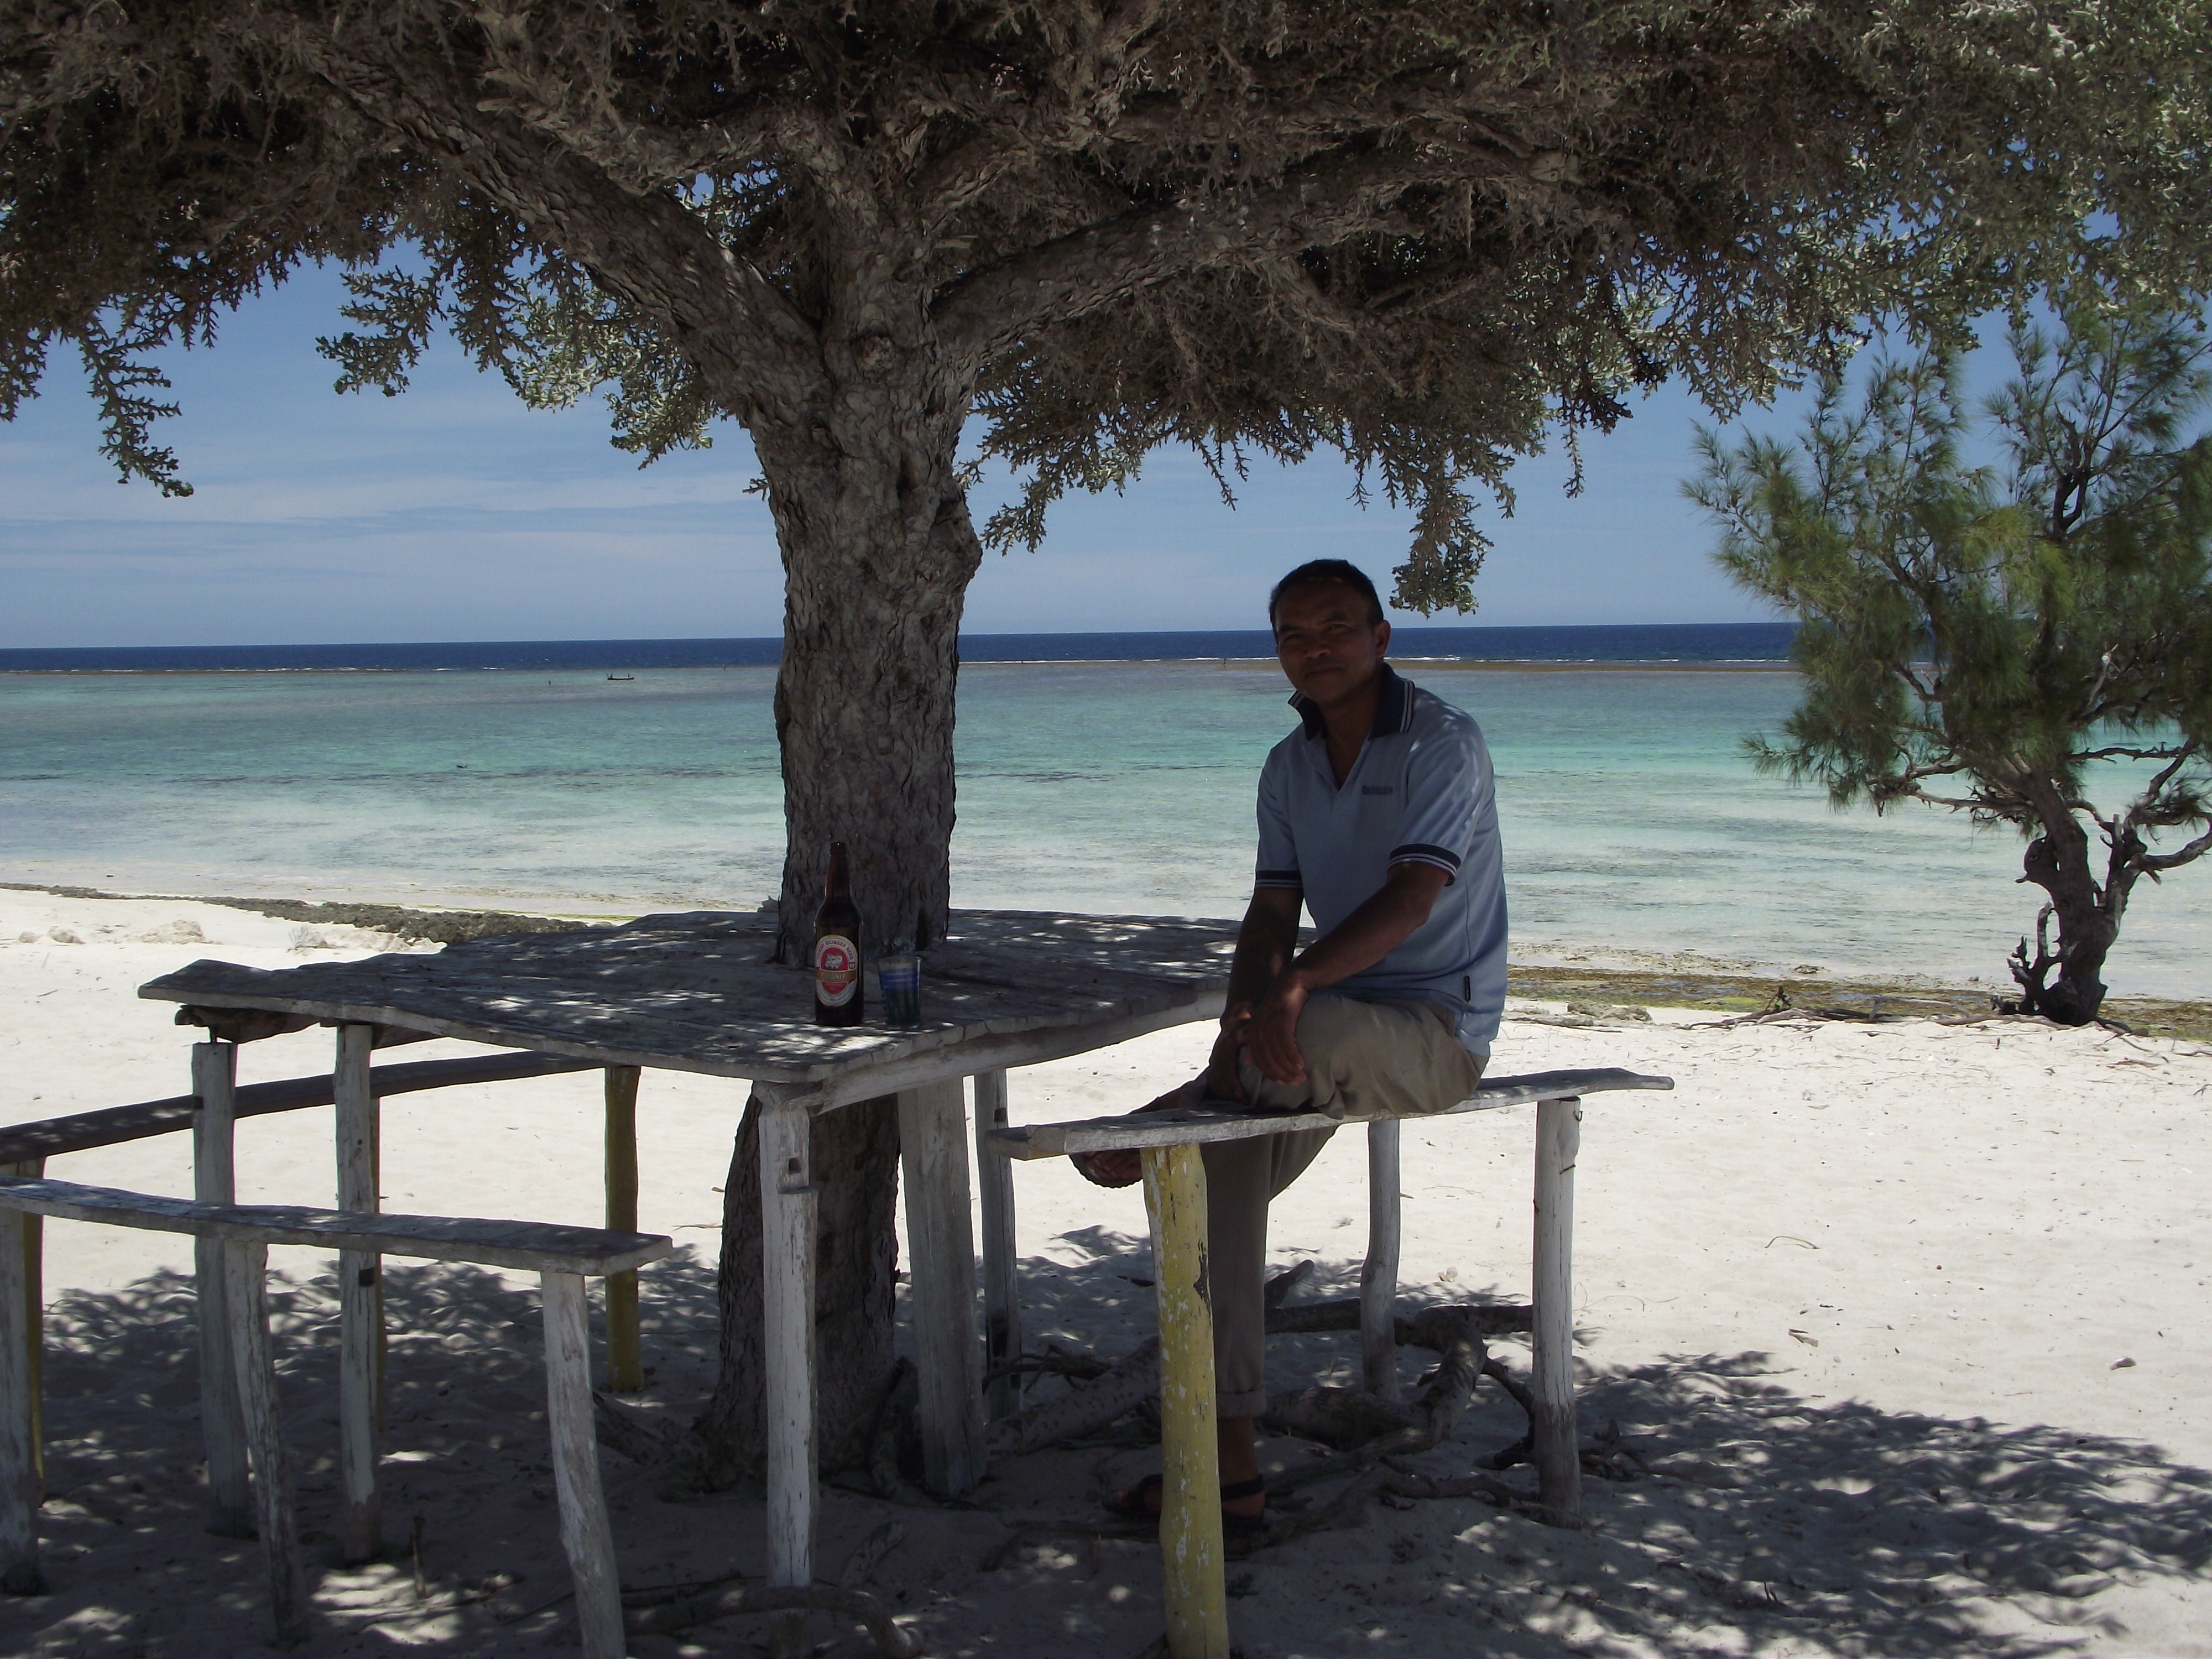
\includegraphics[width=5cm]{articles/Chemins-du-sud/DSCF0321.JPG}
\smallbreak

Allez encore une pirogue, décidément je ne m'en lasse pas..

\smallbreak\smallbreak
\hspace*{-0.65cm}
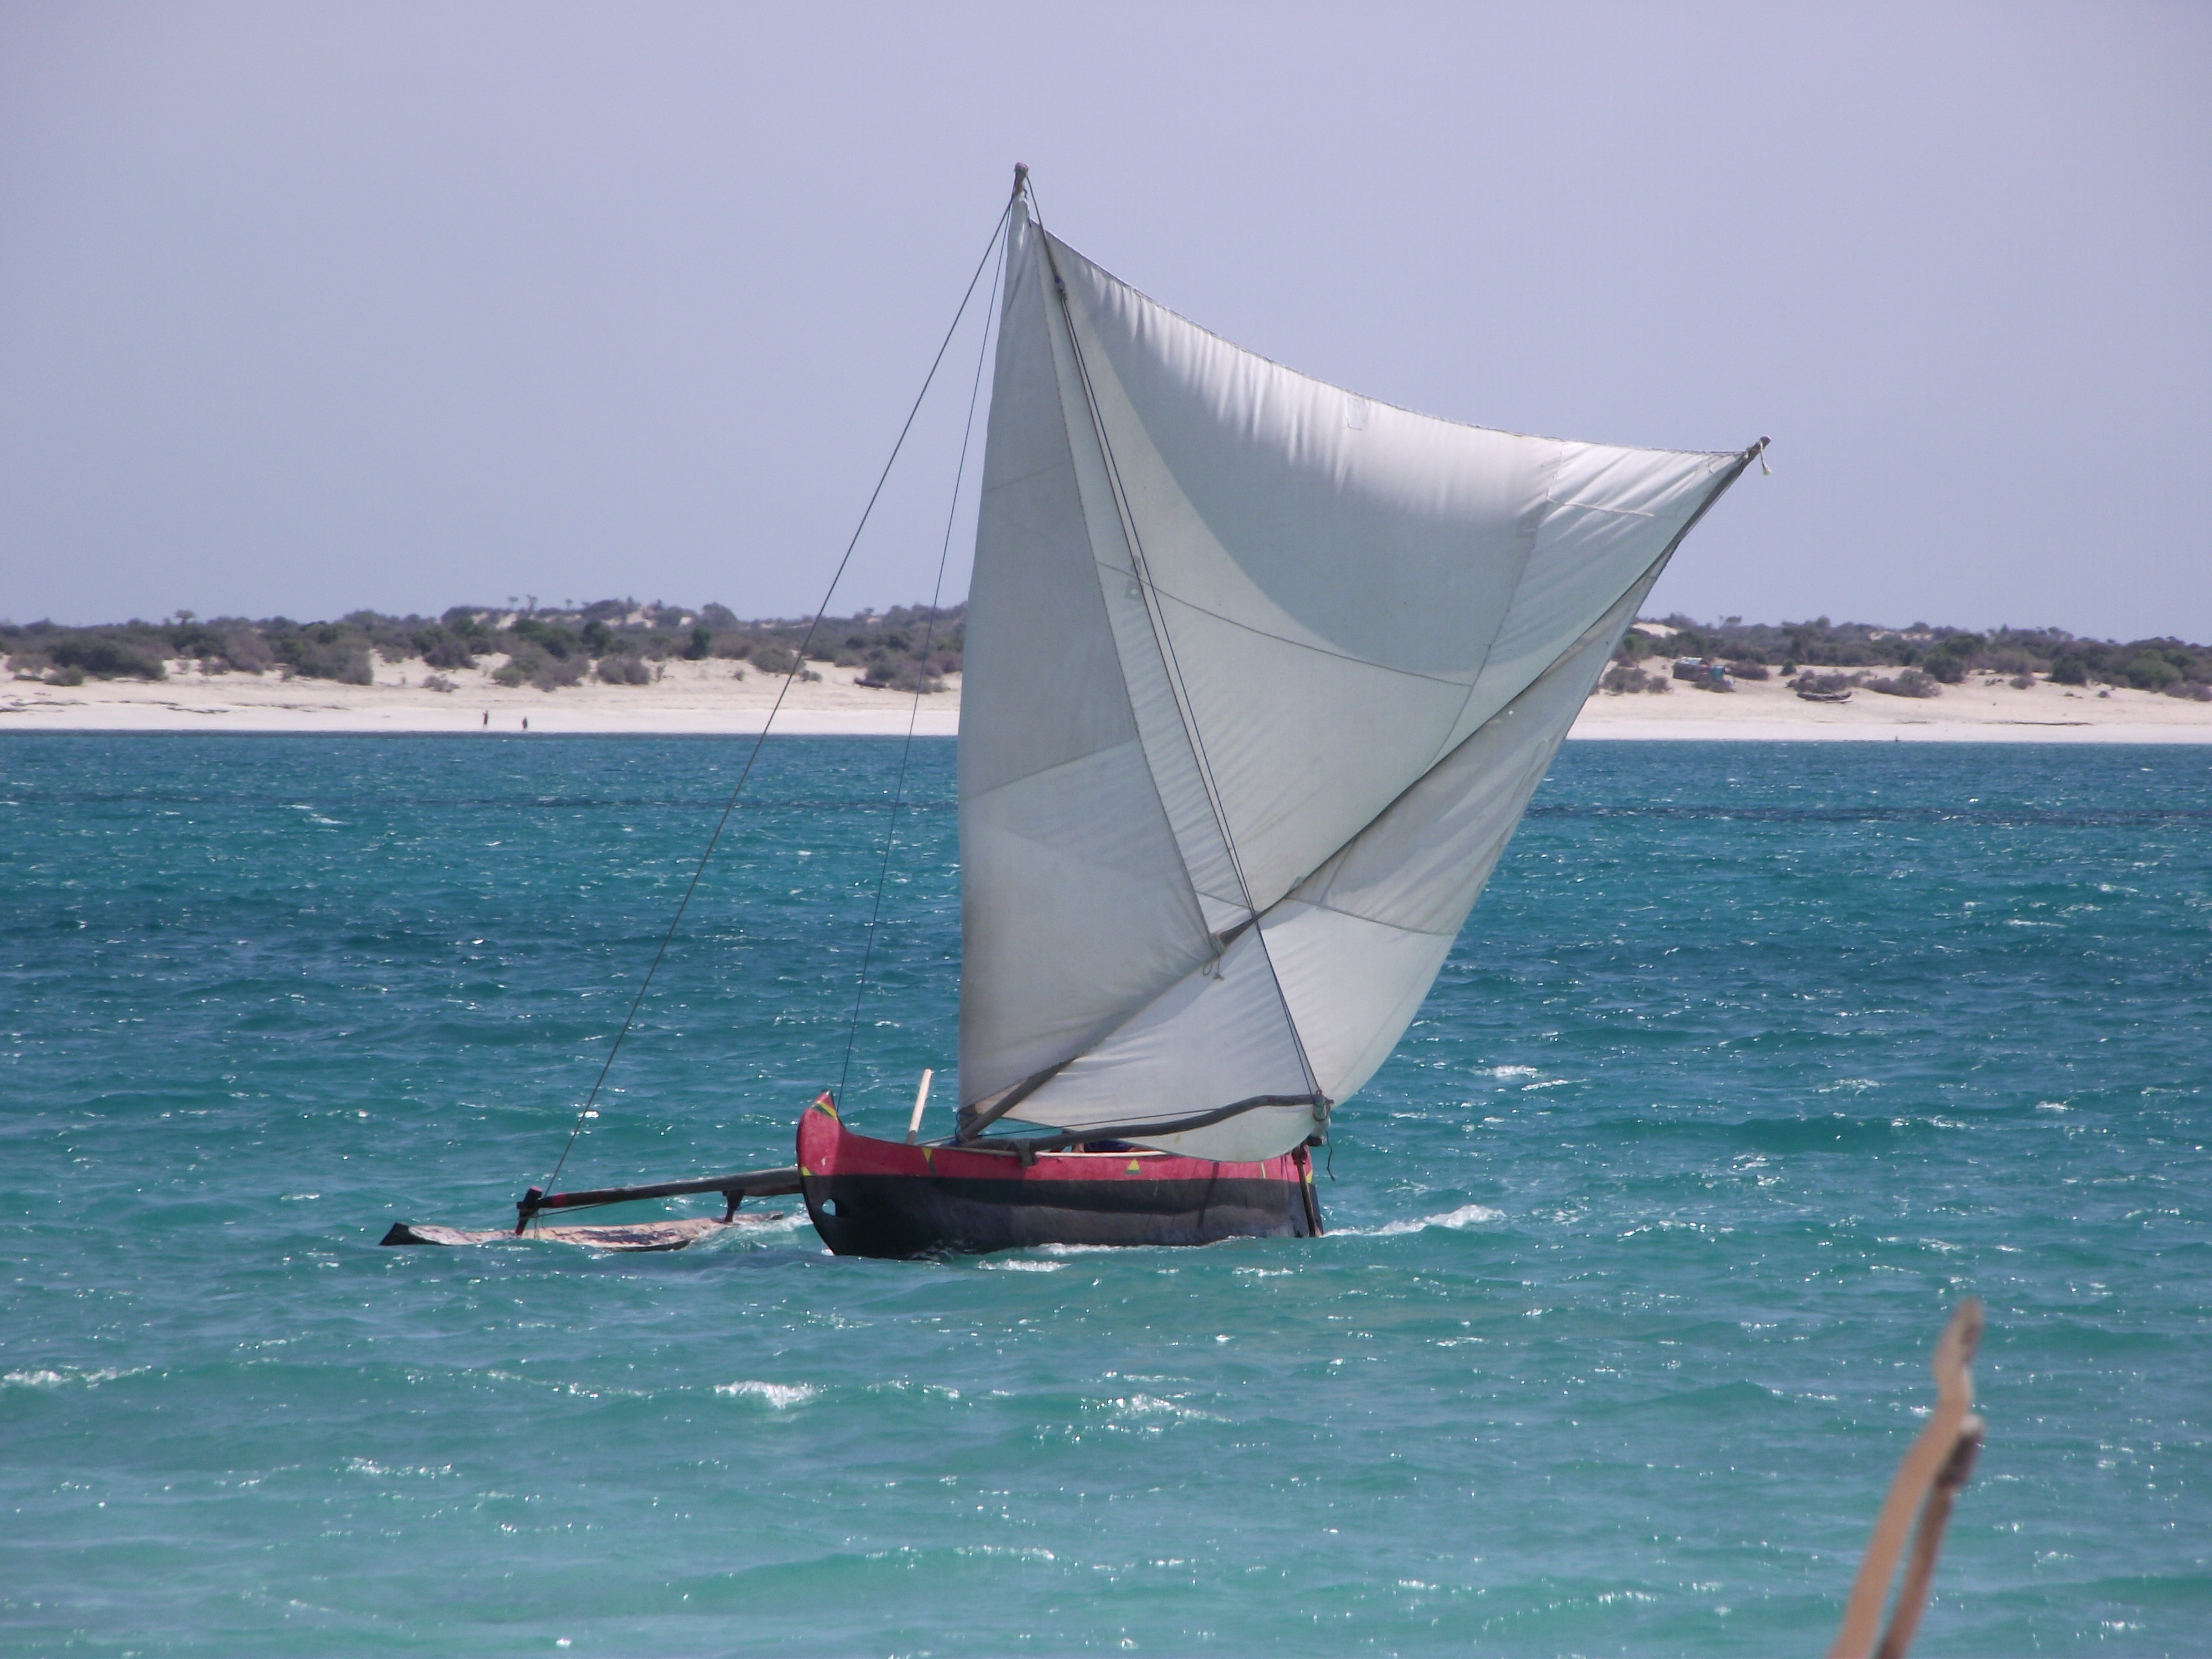
\includegraphics[width=5cm]{articles/Chemins-du-sud/DSCF0338.JPG}
\smallbreak

Et sur la route ? quelques autres 4x4 mais surtout les habitants des villages voisins qui vont travailler la terre, récolter, s'occuper de leur bétail. Ici un char à zébus, moyen de transport le plus répandu dans le coin.

\smallbreak\smallbreak
\hspace*{-0.65cm}
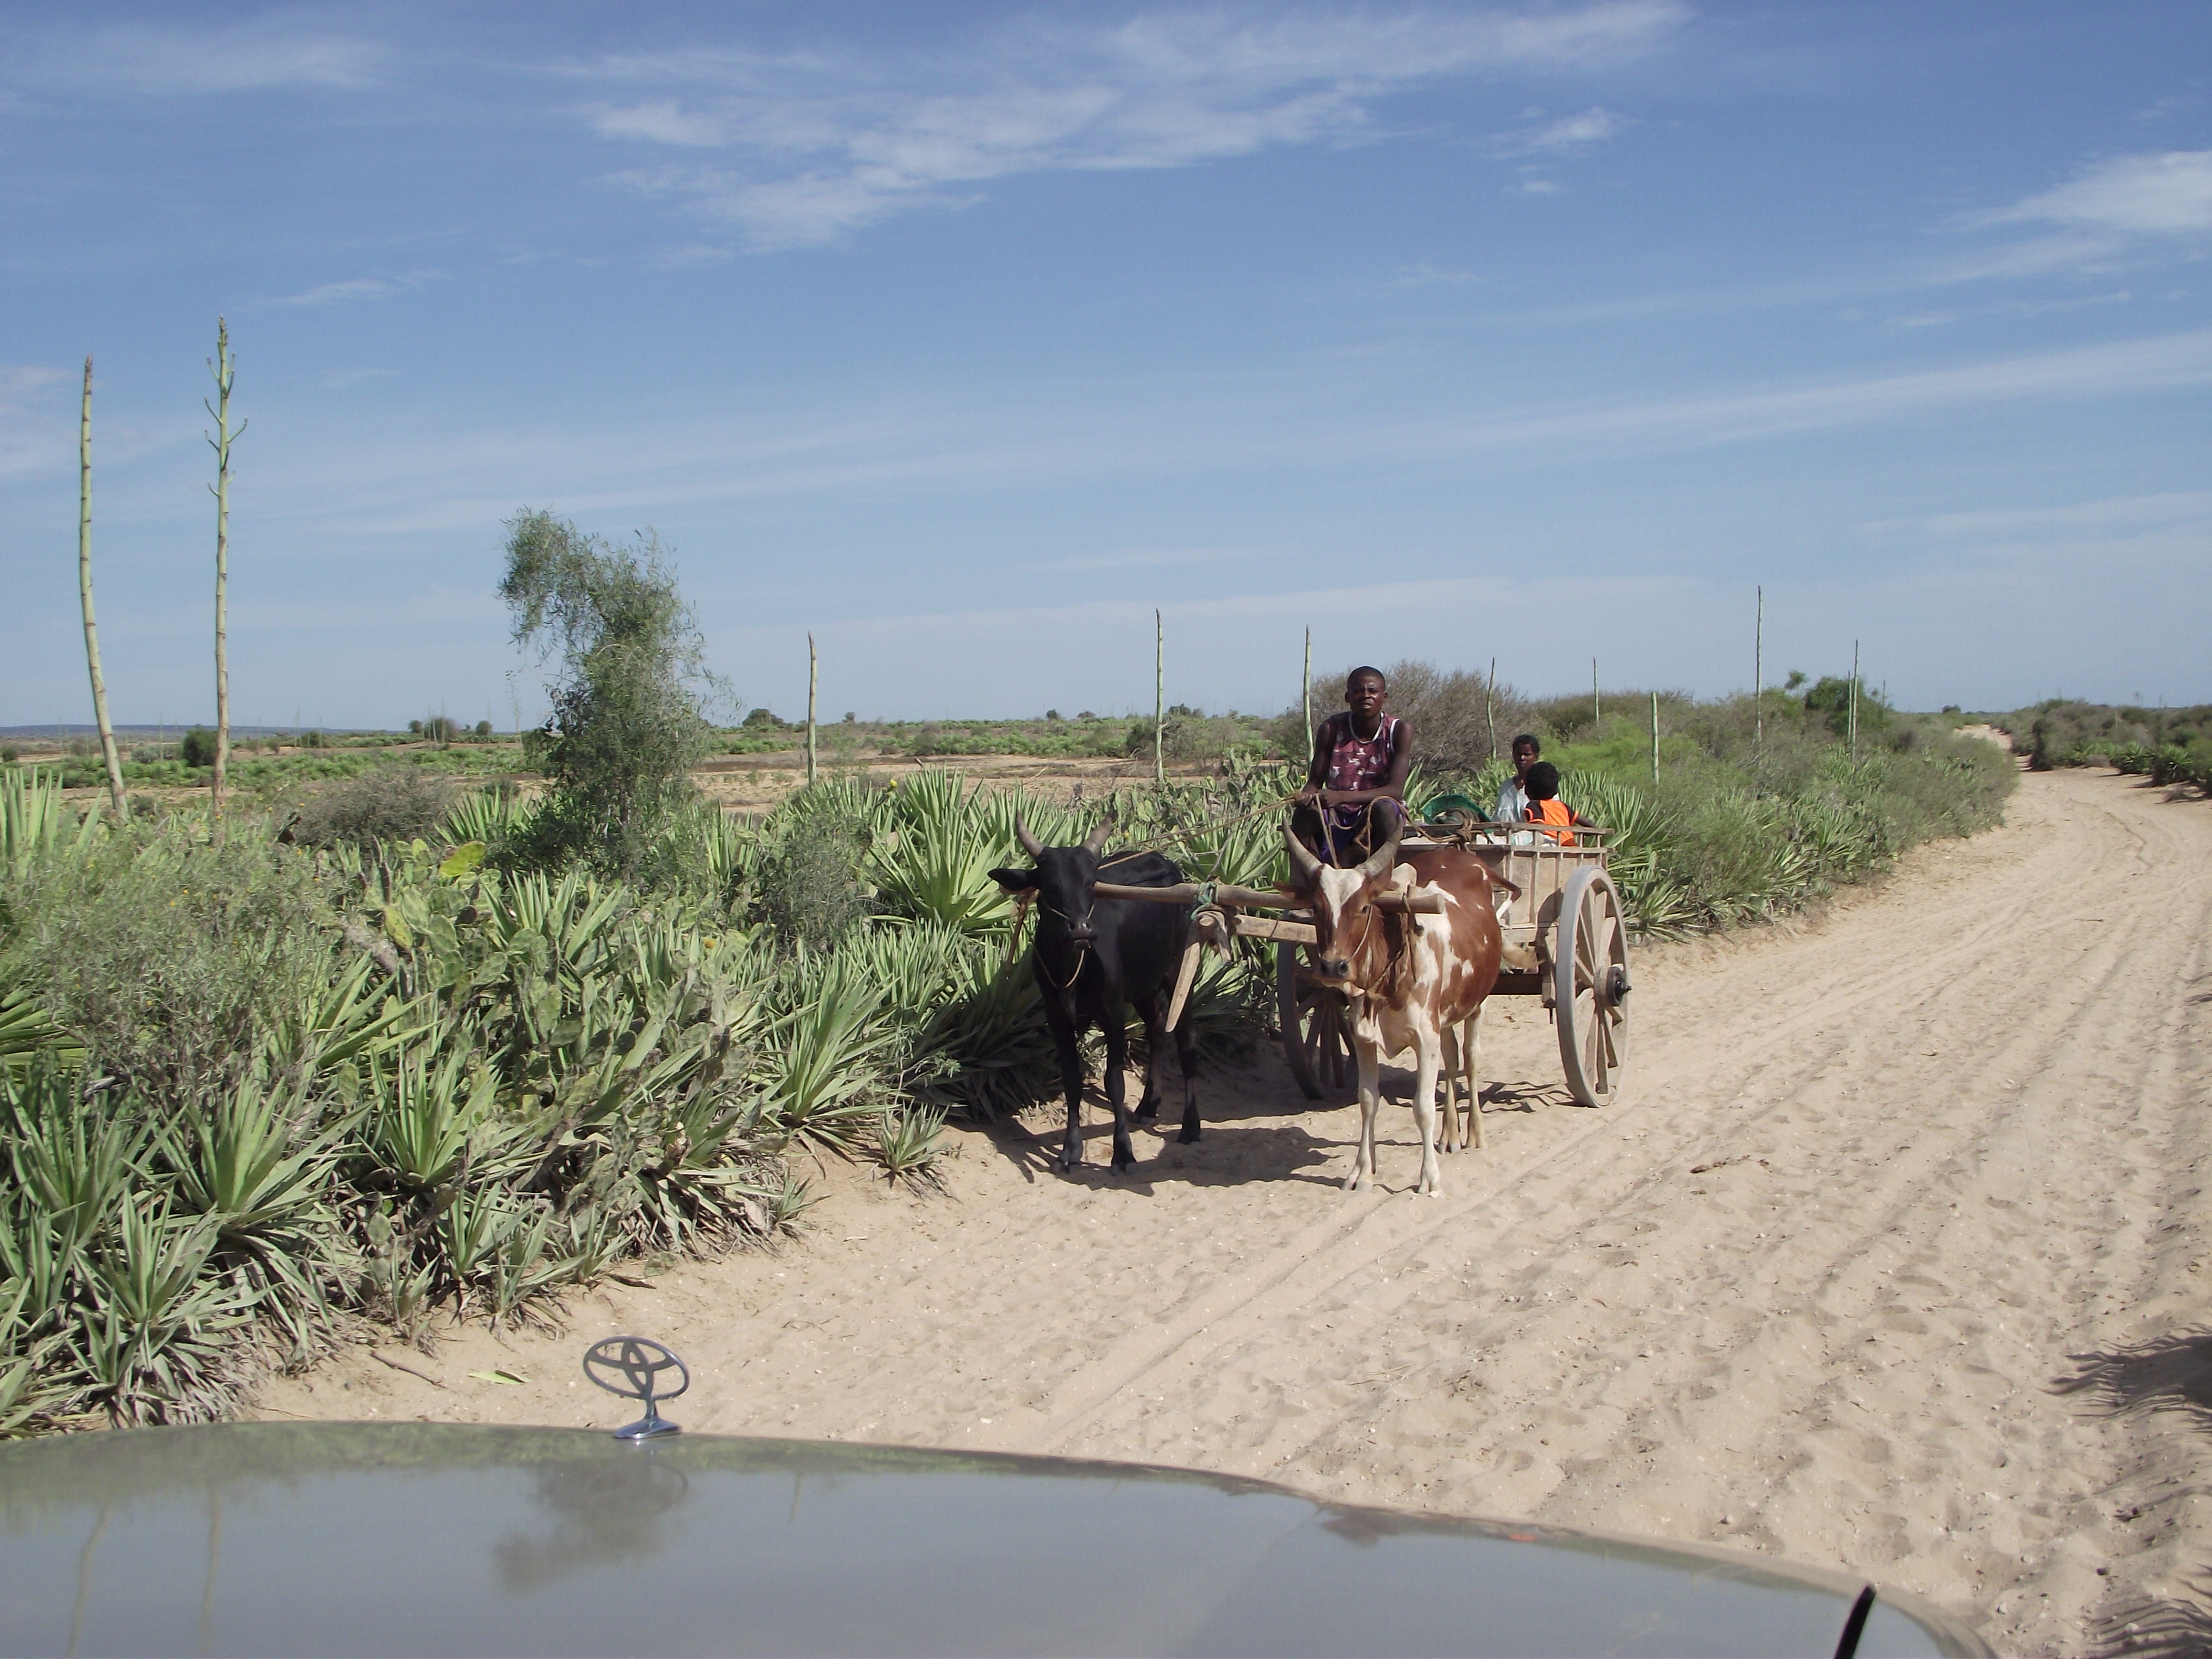
\includegraphics[width=5cm]{articles/Chemins-du-sud/DSCF0344.JPG}
\smallbreak

Rouler, c'est bien joli, mais il faut faire constamment super attention à la route, car en plus des chars à bœufs qui se voient de loin, un grand nombre de tortues traversent la route. Nous n'en avons presque pas vu sur la première moitié alors que c'était un florilège par la suite, parfois 5 tortues en moins de 100 mètres.

\smallbreak\smallbreak
\hspace*{-0.65cm}
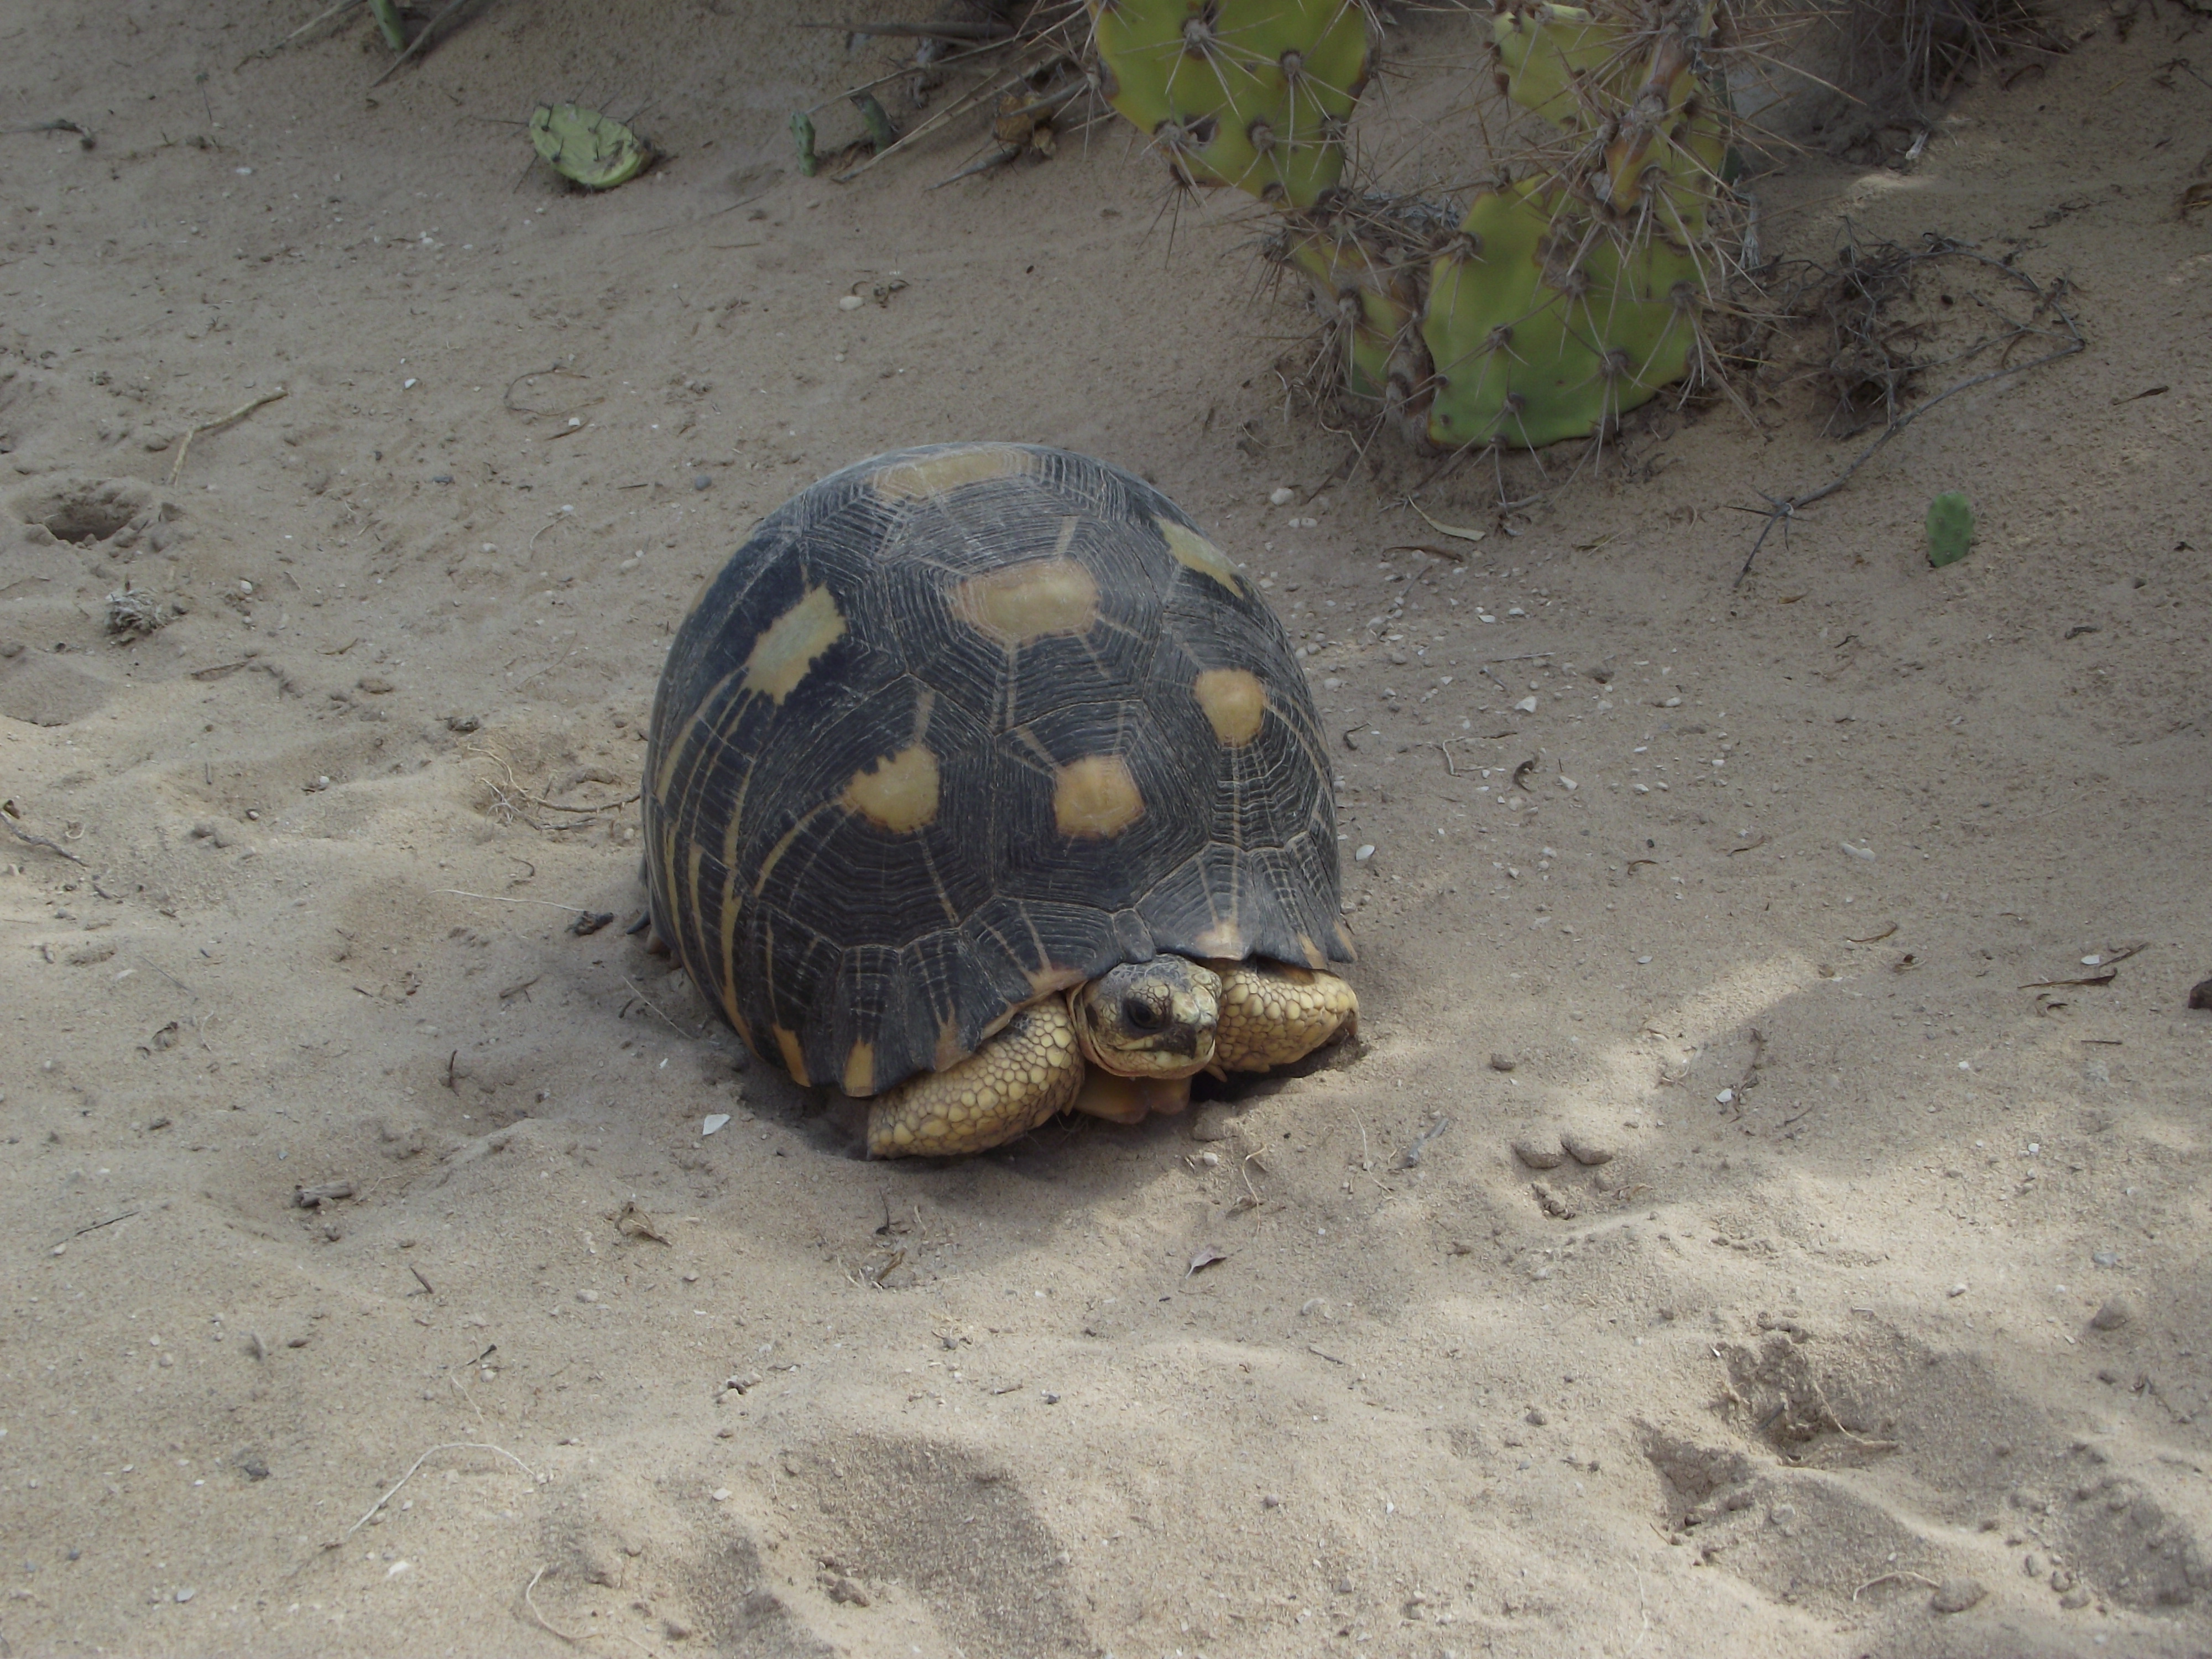
\includegraphics[width=5cm]{articles/Chemins-du-sud/DSCF0345.JPG}
\smallbreak

Au détour d'un câble de frein qui a lâché (notre mécano en chef nous a réparé en moins de 2 secondes en condamnant le freinage d'une roue, tant pis pour le lookeed sur le sable) voici une ch'tite photo de cactus que j'aime bien..

\smallbreak\smallbreak
\hspace*{-0.65cm}
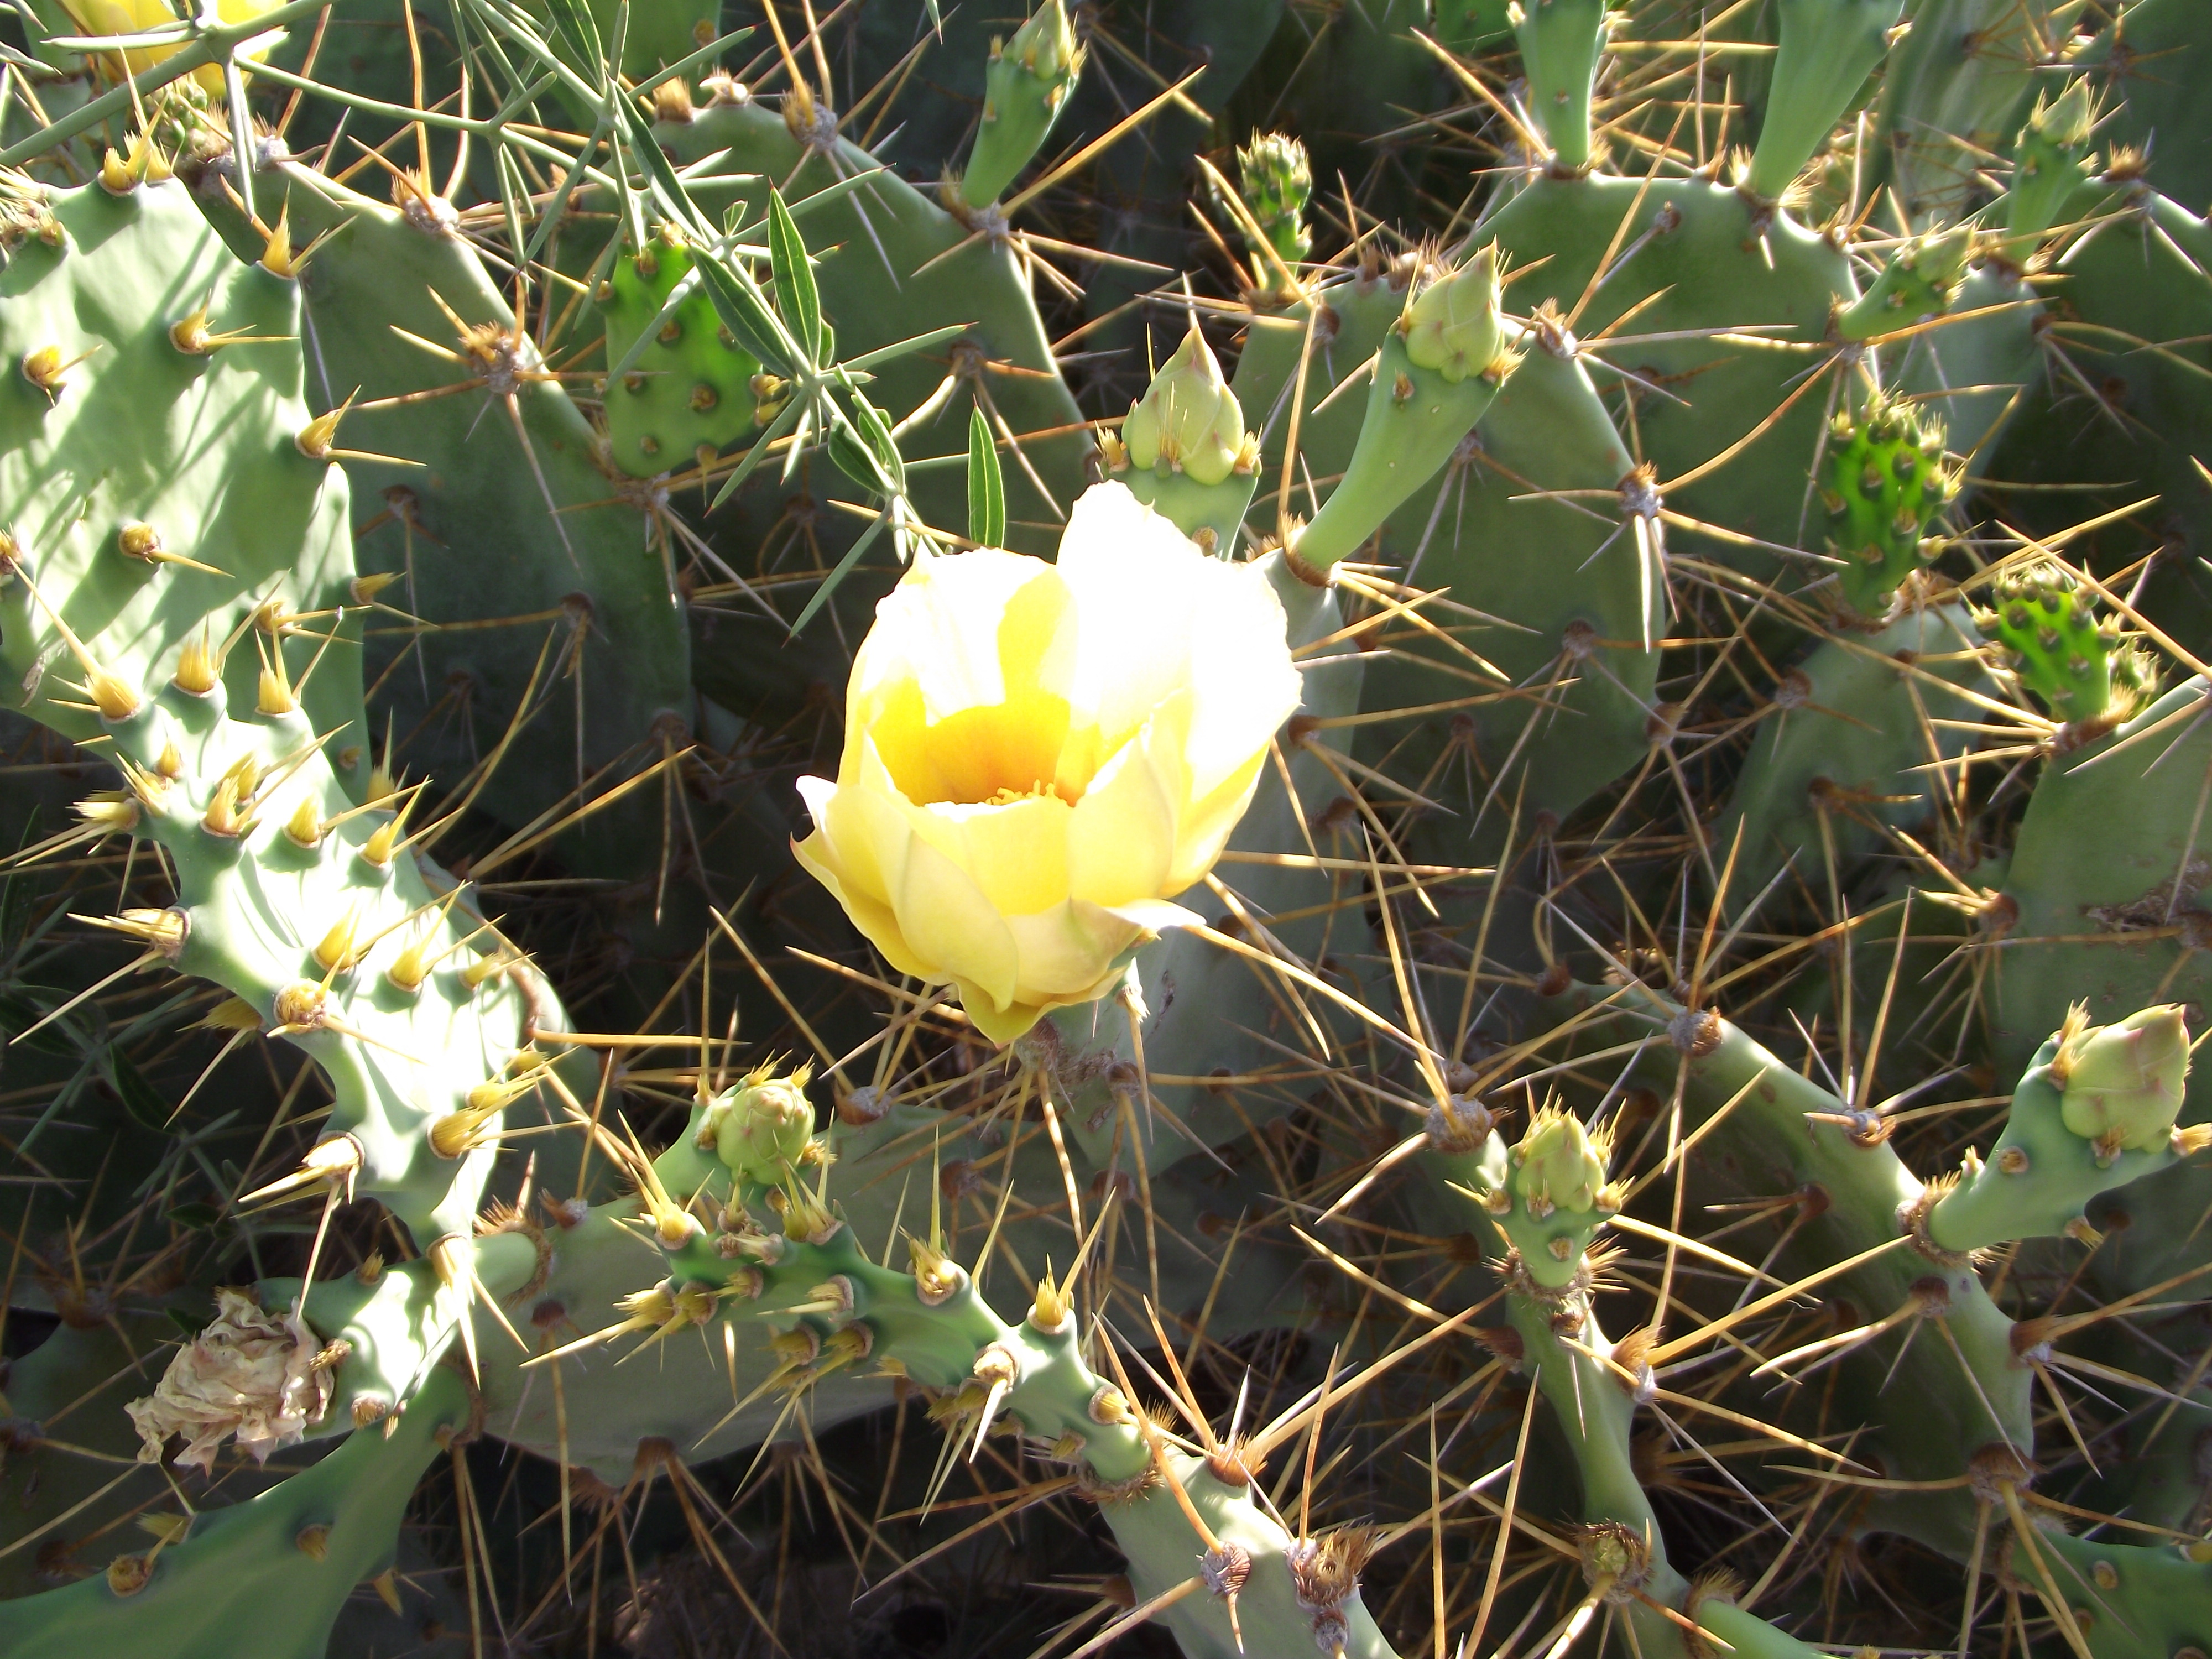
\includegraphics[width=5cm]{articles/Chemins-du-sud/DSCF0354.JPG}
\smallbreak

Le bolide en question :

\smallbreak\smallbreak
\hspace*{-0.65cm}
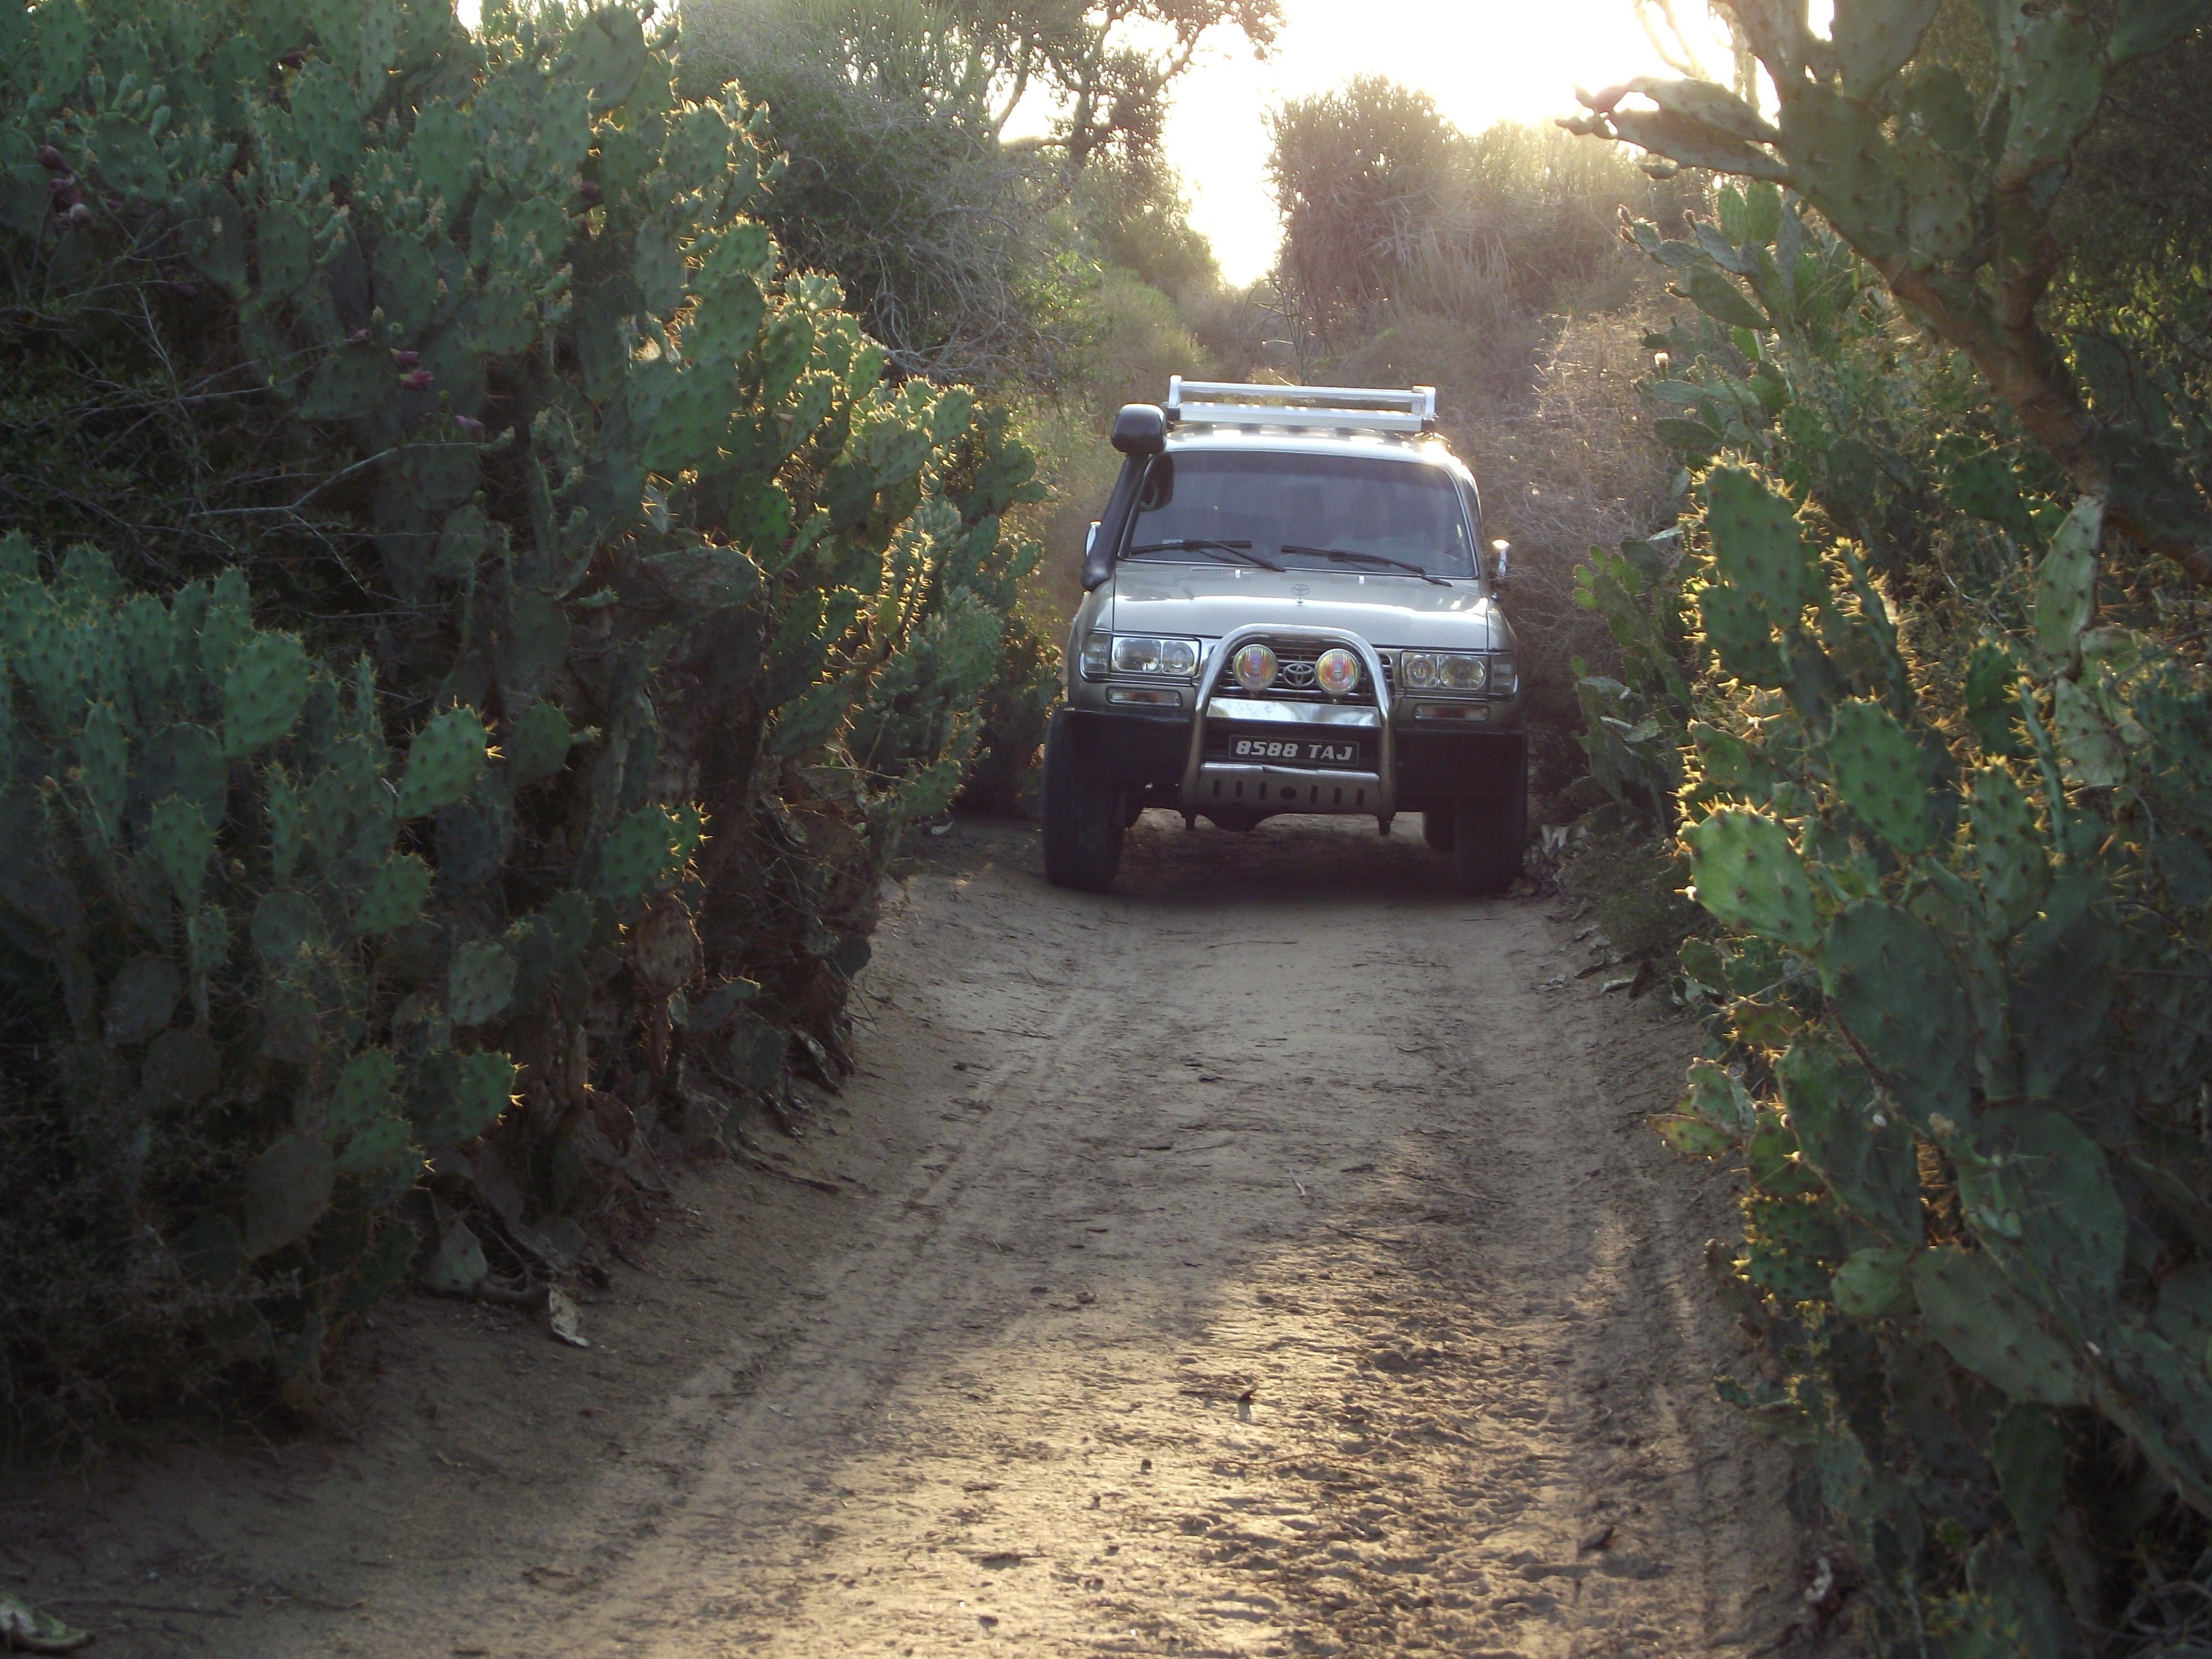
\includegraphics[width=5cm]{articles/Chemins-du-sud/DSCF0358.JPG}
\smallbreak

La piste était parfois vraiment sport, ici un passage assez étroit.

\smallbreak\smallbreak
\hspace*{-0.65cm}
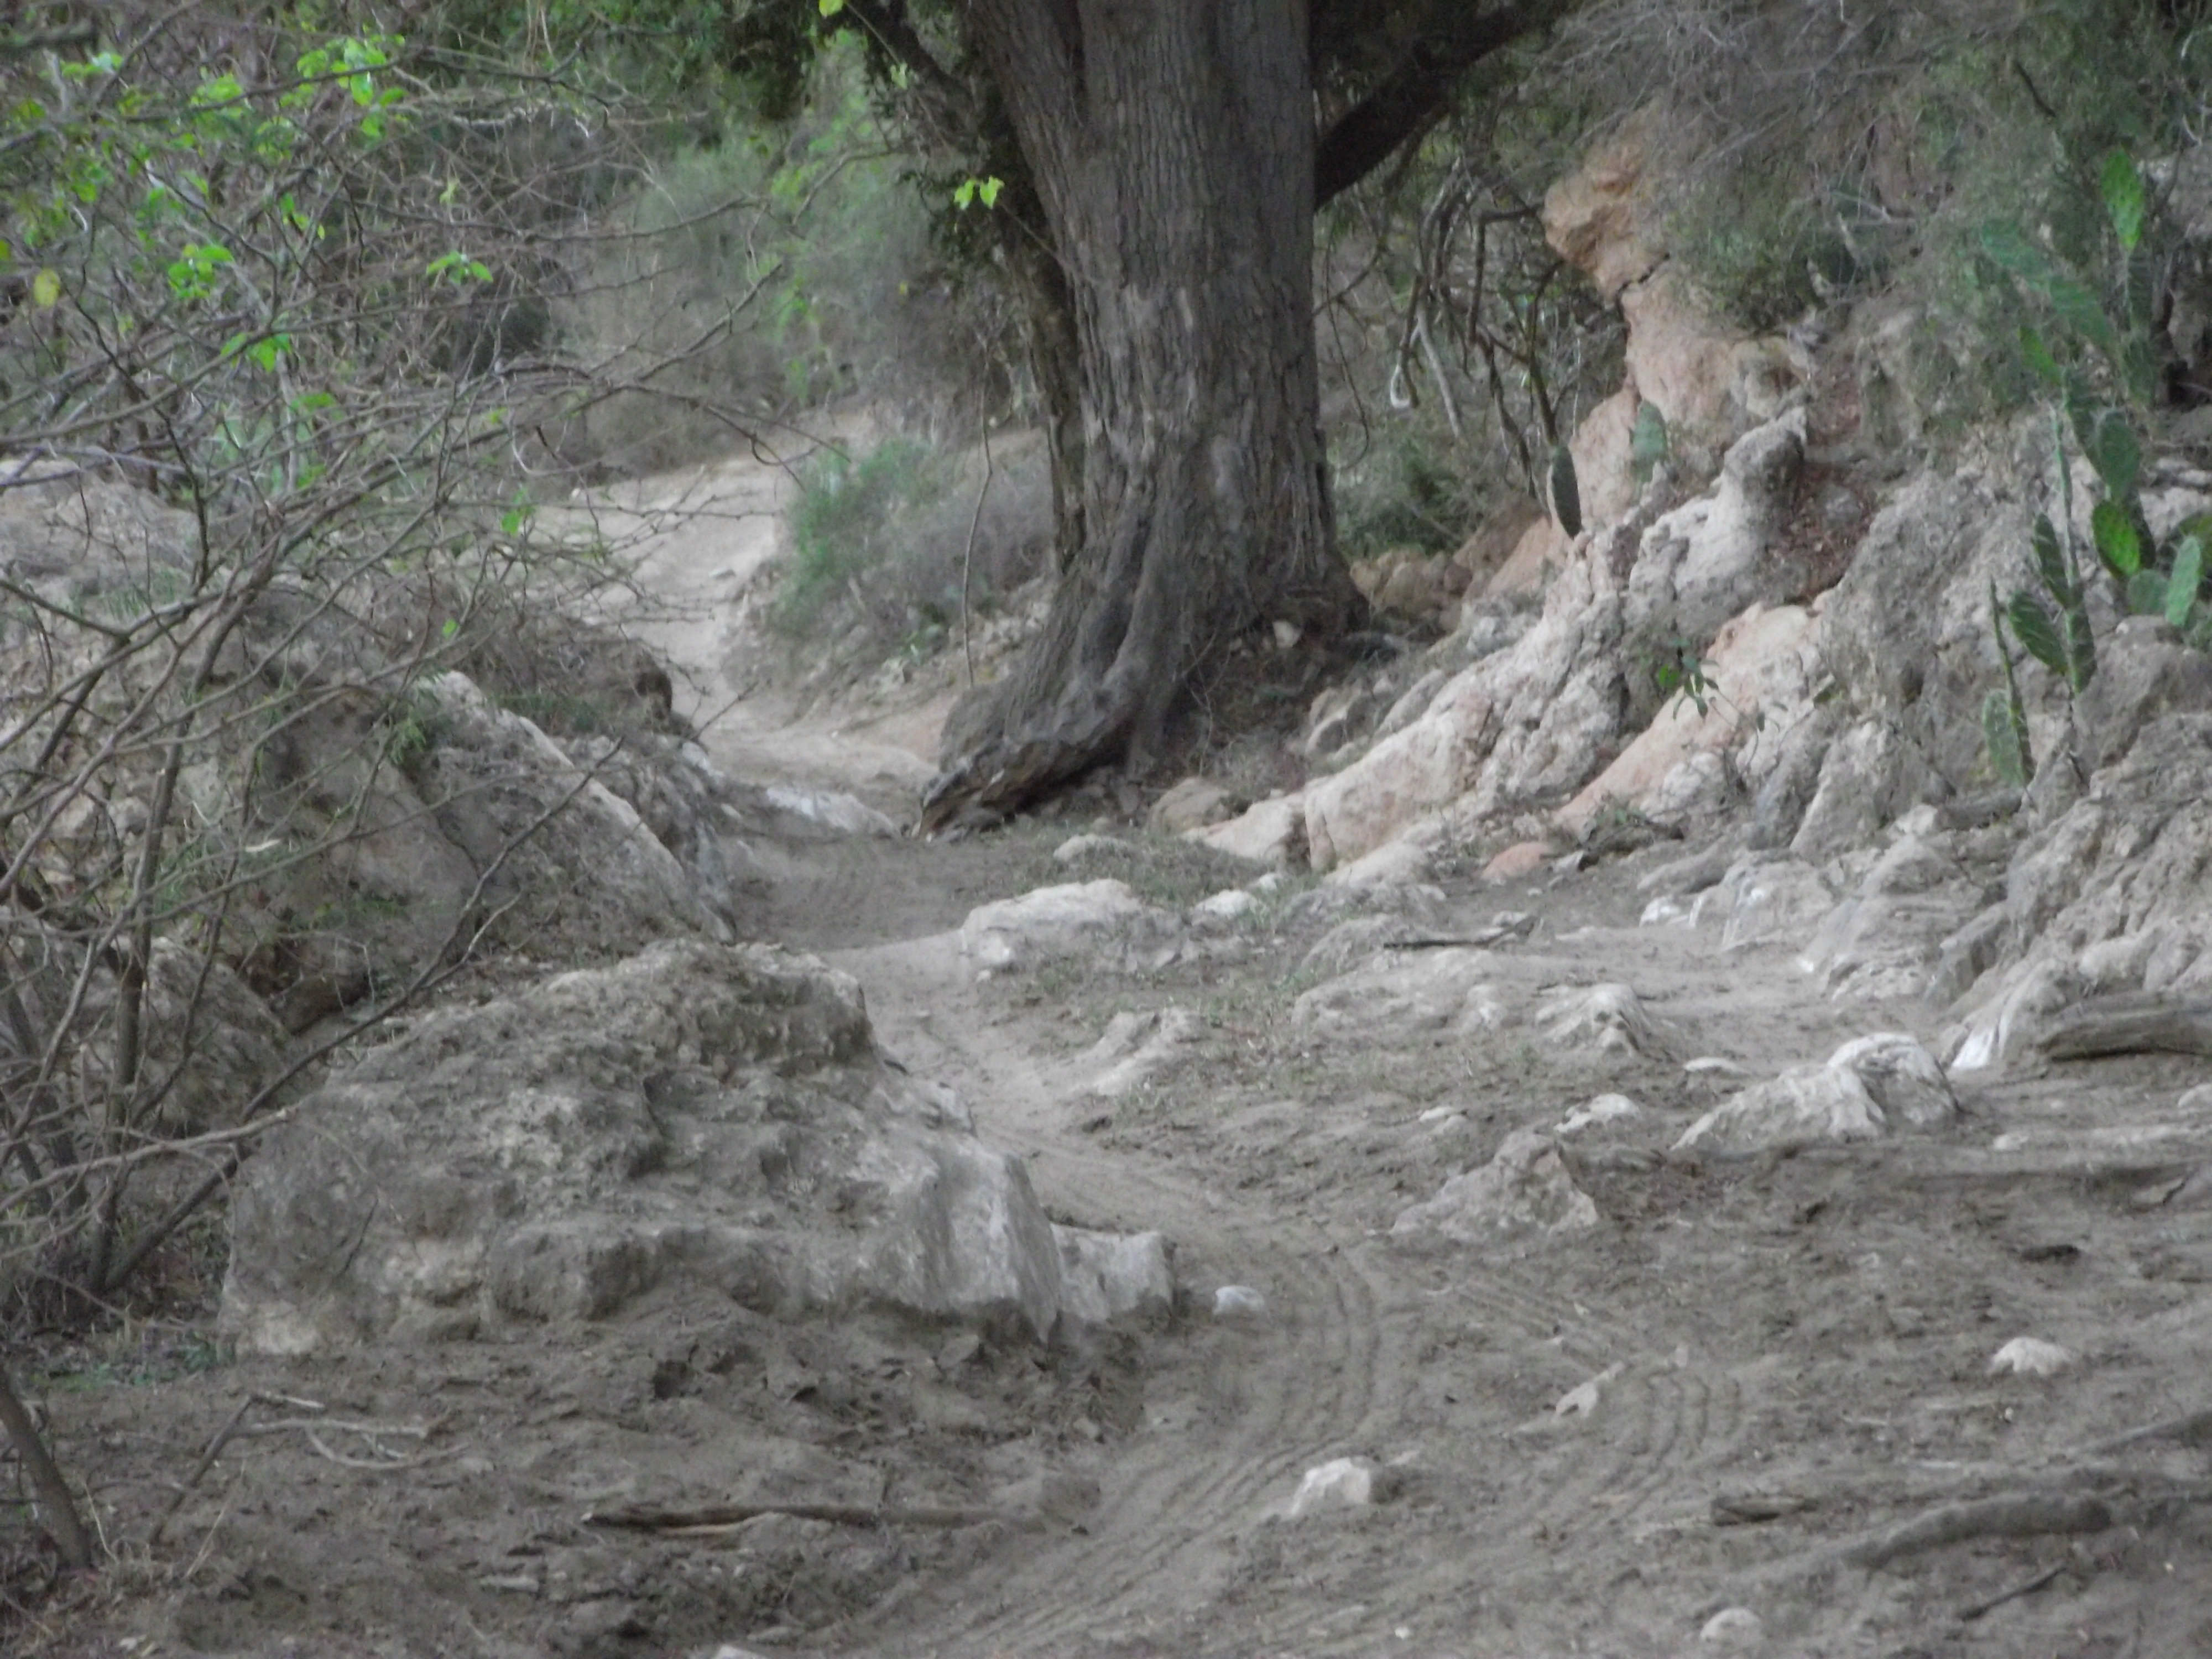
\includegraphics[width=5cm]{articles/Chemins-du-sud/DSCF0362.JPG}
\smallbreak

Et puis c'est l'arrivée sur Fort Dauphin, qui a certes de jolies plages, mais que j'ai trouvée assez terne. En fait je pense que je suis passé à coté de cette ville, il semblait y avoir plusieurs endroits magnifiques à visiter notamment un tour de pirogue à faire pour contourner une baie, mais différents problèmes pour gérer mon retour sur Tana avec Air Mada (mora mora..) m'ont empêché d'en voir plus. Même les grandes institutions de l'île sont soumises aux aléas, au fatalisme. Un jour il n'y a plus de places, le lendemain les places ont toujours existé mais impossible de payer, perte de temps.. Mada !

Une plage de Fort Dauphin.

\smallbreak\smallbreak
\hspace*{-0.65cm}
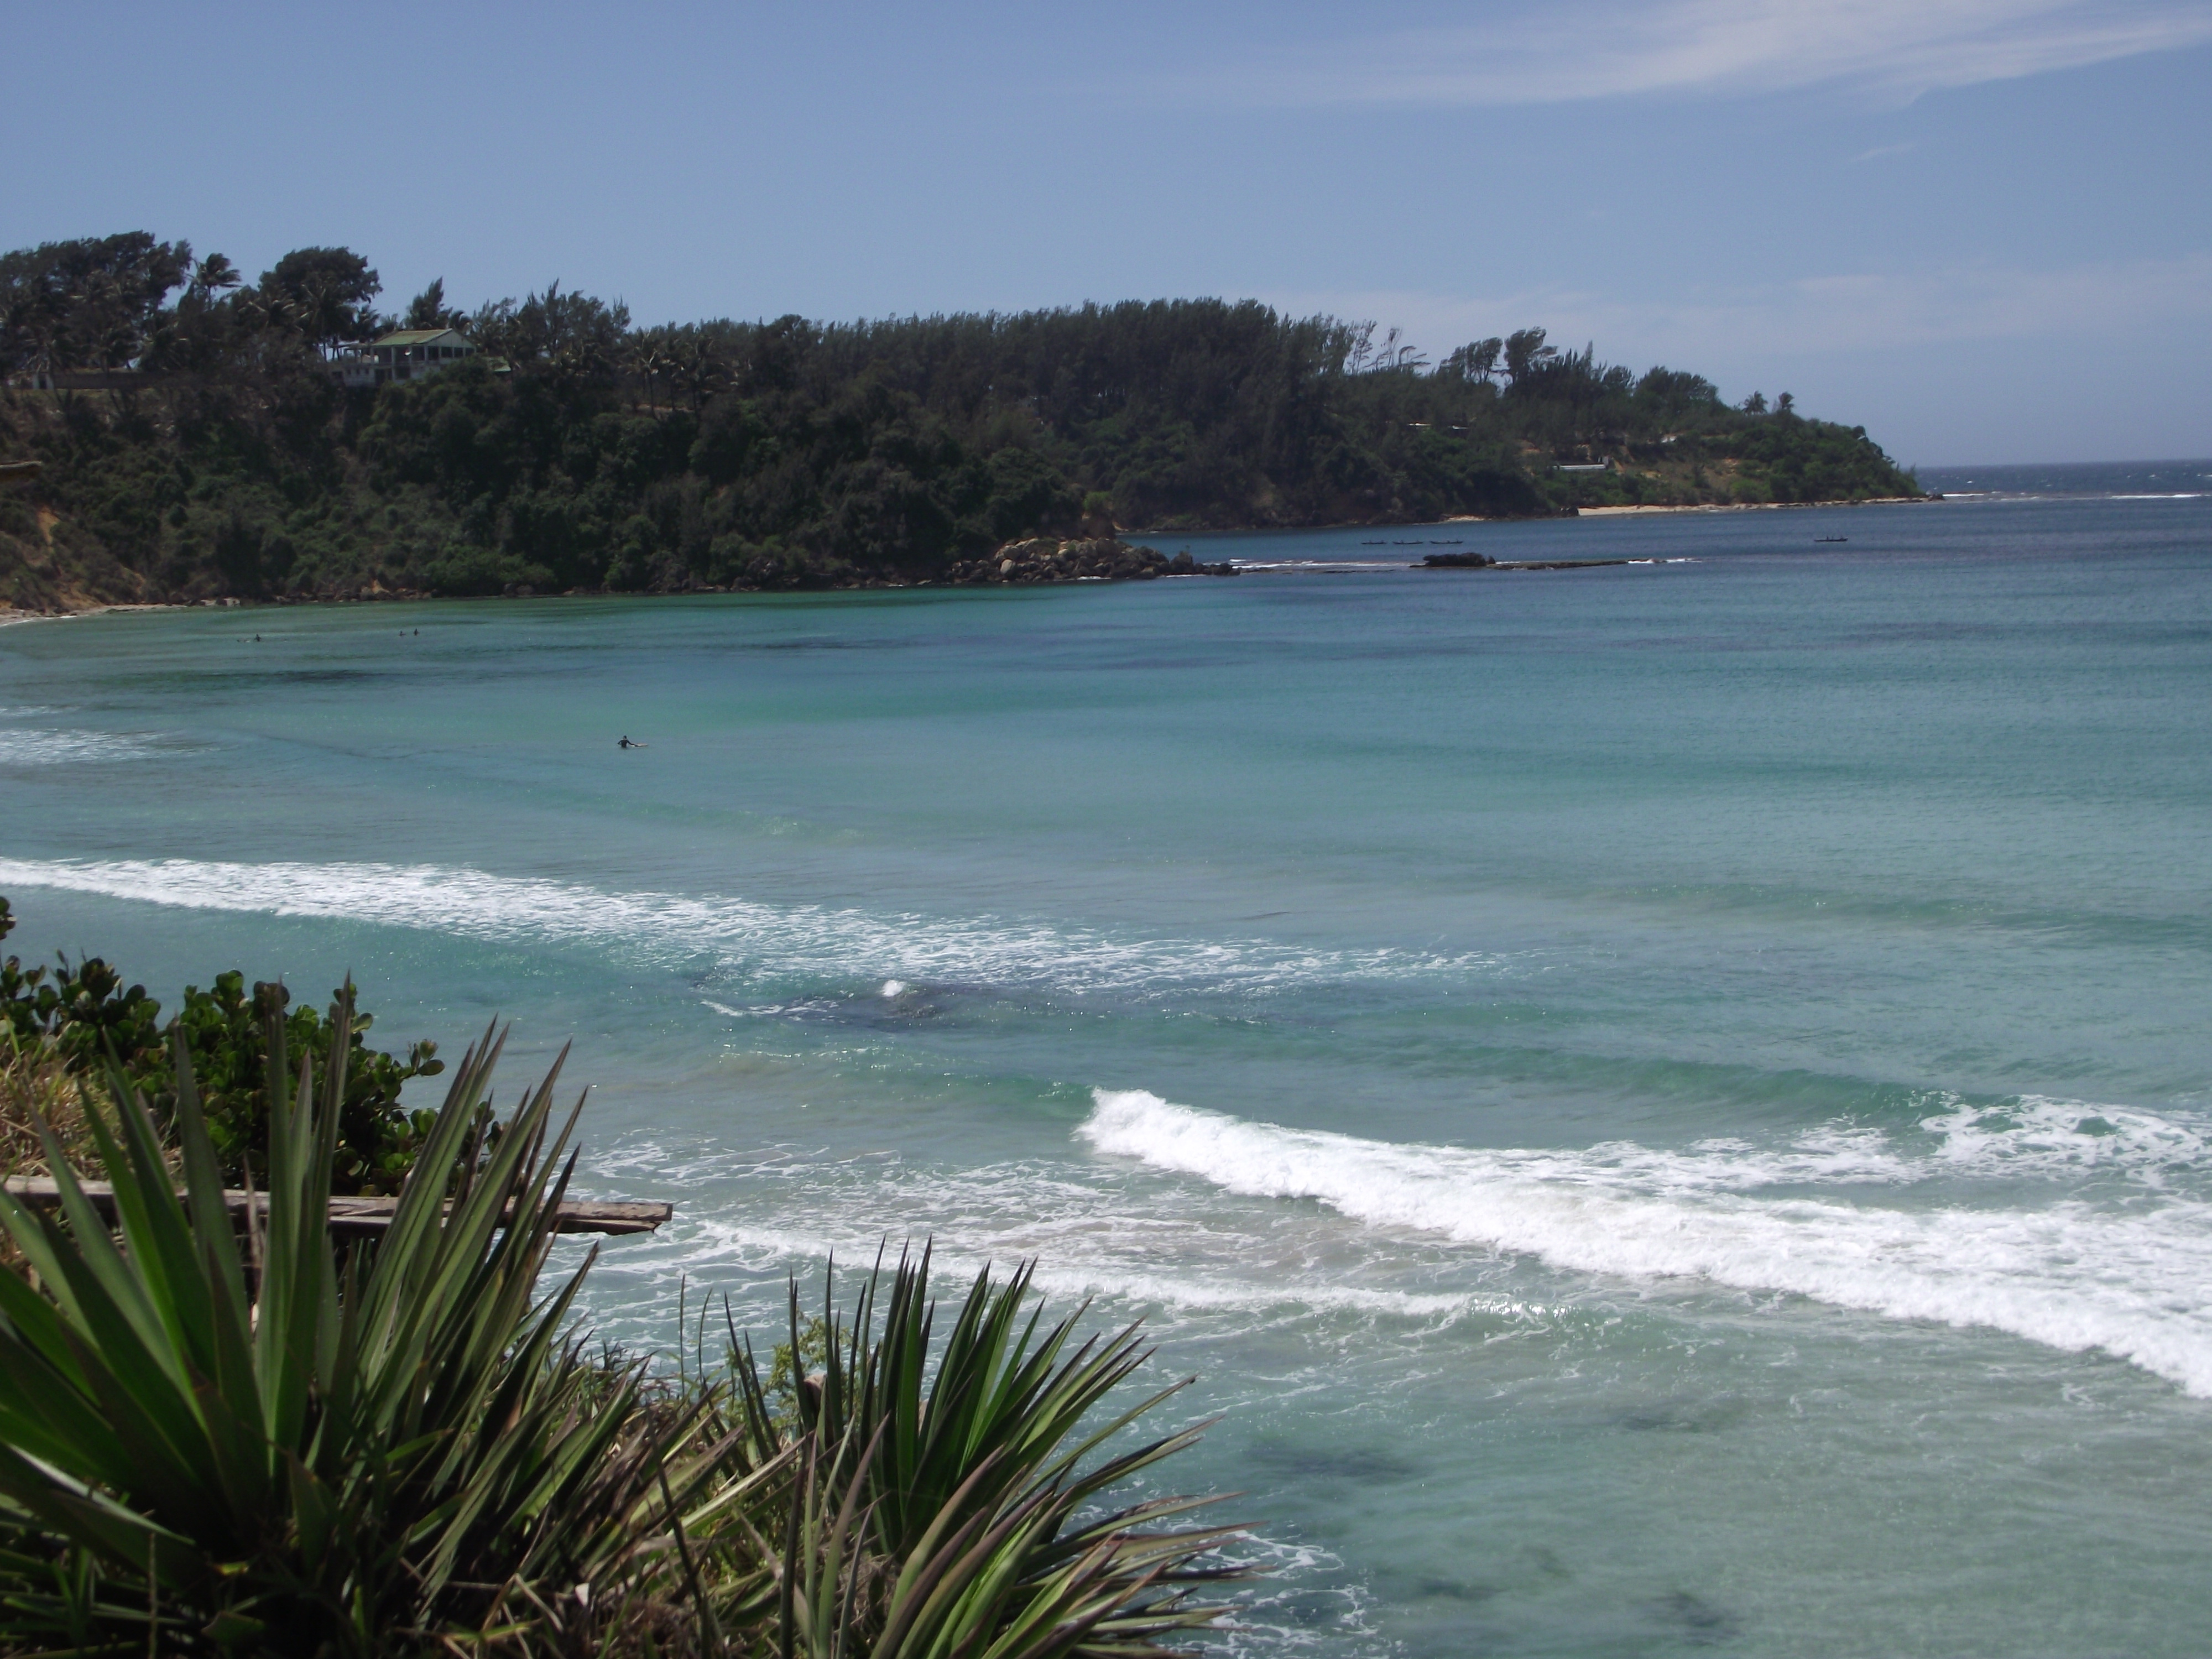
\includegraphics[width=5cm]{articles/Chemins-du-sud/DSCF0375.JPG}
\smallbreak

Me voici maintenant revenu à Tana après avoir enfin pu trouver et payer ma place dans un coucou, mon programme pour la suite est de monter vers le nord tranquillement, les routes étant moins bonnes que vers le sud (ça promet !). Je redescendrai ensuite par un deuxième vol intérieur du Nord vers Tana, seule solution pour être sûr du retour.

Je vous laisse sur une question.. Le zébu ressemble étrangement à une vache, et pourtant il s'adapte beaucoup mieux à ces chaleurs, alors pourquoi n'a t-il jamais soif ?

\end{multicols}

\bigskip
\textbf{\textsc{Commentaires}}

\medskip
Titou a écrit le 26 nov. 2010 :
\begin{displayquote}
Yeah pti Dud !
Ralala ça donne vraiment envie de partir et de te rejoindre quand on te lit et qu'on voit toutes ces magnifiques photos !
Dire que nous on est tous comme des glands à regarder par la fenêtre pour savoir si il neige ou pas\dots Enfin profites en à fond comme tu le fais si bien, et continues de faire gaffe à toi !
PS 1: Pour le Zébu bah normal, quand zébu zé plus soif :-)
PS 2: J'ai adoré le caméléon\dots qui est très mora mora lui aussi :p
A plutch
biz.
\end{displayquote}

\medskip
Chachou a écrit le 27 nov. 2010 :
\begin{displayquote}
Coucou ti dud,
Ça ressemble pas à une saison des pluies question météo! Ça fait rêver! Tes photos sont trop belles.
Pour le Zébu : Généralement, le poil est de couleur claire, lui permettant de supporter la chaleur. La peau est ample, voire lâche sous le cou : elle augmente la surface, permettant un meilleur échange thermique.
Une bosse graisseuse rehausse le niveau du garrot, elle constitue une réserve calorique qui leur permet de supporter des périodes de "vaches maigres". C'est wikipédia qui l'a dis :-)
Gros bisous, profite!
\end{displayquote}

\medskip
Sarah a écrit le 28 nov. 2010 :
\begin{displayquote}
Salut Etienne!
Génial toutes ces photos et les détails!
on s'y croirait !
j'adore particulièrement la ptite Paola, la table de restau sur la plage et le poisson fraichement pêché, mmmmmmmm\dots.
Profites bien ma caille ;)
Sarah T.
\end{displayquote}

\medskip
Etienne a écrit le 28 nov. 2010 :
\begin{displayquote}
@Sarah : Super de te voir passer dire bonjour ! Je dois dire que j'ai aussi particulièrement apprécié ce poisson grillé avec vu sur le lagon, et si j'en crois ce qu'on me dit j'ai pas finis d'en prendre plein la vue avec les paysages maritimes au nord.. plages, lagon, cocotiers.. les Maldives n'ont qu'à bien se tenir !
@Titou et Chachou, un point partout pour la réponse humoristique et la réponse scientifique\dots Vous savez à laquelle je pensais ;)
\end{displayquote}

\medskip
El Duderiño a écrit le 28 nov. 2010 :
\begin{displayquote}
Salut vieux,
les taxi-brousses, c'est comme les collectivos en Amérique Latine\dots, c'est juste le nom qui change, mais le principe reste le même ;-)
Par contre ton 4x4 a quand même l'air plus solide que ceux sur le Salar d'Uyuni
Sinon tu loges où en général ? je doute qu'il y ait beaucoup de "hostals de fiesta" sur l'île\dots ;-)
Profite bien man
A+
El Duderiño.
\end{displayquote}

\medskip
Tatid a écrit le 29 nov. 2010 :
\begin{displayquote}
Mort de rire le "mora mora", si toi tu perds patience, qu'est-ce que ce serait pour moi :-D
En tous cas, je me joins aux autres pour dire que les photos sont magnifiques et je suis d'ac avec Fab pour dire que le caméléon fait très "mora mora" aussi !!
Profite l'ami !
\end{displayquote}

\medskip
Tatid a écrit le 29 nov. 2010 :
\begin{displayquote}
Et au fait, un truc de geek, faudra que tu thunes ton flux RSS histoire de mettre dans le corps du flux RSS l'article entier et pas seulement "L'article de blog concernant Chemins du sud" ;-)
\end{displayquote}

\medskip
Dova a écrit le 29 nov. 2010 :
\begin{displayquote}
Et nous qui nous inquiétions pour toi!!!
Vraiment pas de quoi :)
A te lire et à voir tes photos, tout va pour le meilleur des monde.
C'est grandiose, je suis jalouse\dots Vivement mon tour.
En fait, ton retour ne saurait tarder?! Encore un peu de repis. Kiffes bien et on t'attend ici avec la neige.
Muitos beijinhos.
\end{displayquote}

\medskip
Dodo a écrit le 30 nov. 2010 :
\begin{displayquote}
Ah bah c'est du joli !! Je vois que y'en a qui se font plaisir pendant que d'autres se les p**** à Orléans !
En tout cas belles photos, tu nous vends du rêve\dots Et uiiiii !! A quand ta prochaine rencontre avec les Makis ou autres lémuriens ?? J'adore ces bestioles :D
Bon trip ;)
\end{displayquote}

\medskip
Papa a écrit le 5 déc. 2010 :
\begin{displayquote}
profite bien du soleil. Ici l'hiver bat son plein.
\end{displayquote}

\medskip
Flo a écrit le 6 déc. 2010 :
\begin{displayquote}
Ca donne bien envie de repartir tout ça!!!
Ramène-nous un peu de soleil et de chaleur dans ton sac à dos!
Bonne continuation et à bientôt l'artiste :)
\end{displayquote}

\vfill

